\part{组合学}

\chapter{排列与组合}
\section{计数原理与排列组合}
\subsection{排列、组合的基本概念}
从若干个元素中取出几个或全部的一种排法,
称作是一个\DefineConcept{排列}(permutation).
例如,从\(a,b,c,d\)四个字母里一次取出两个的排列数有12个,即\begin{gather*}
%@Mathematica: SolvePermutationProblem[list_, n_] := Module[
%					{results},
%					results = Permutations[list, {n}];
%					Print[StringForm[
%						"从`1`这`2`个字母里一次取出`3`个的排列数有`4`个:\n`5`",
%						list, Length[list], n, Length[results], results
%					]];
%				]
%@Mathematica: SolvePermutationProblem[{a, b, c, d}, 2]
	ab, \quad
	ac, \quad
	ad, \quad
	bc, \quad
	bd, \quad
	cd, \\
	ba, \quad
	ca, \quad
	da, \quad
	cb, \quad
	db, \quad
	dc;
\end{gather*}
其中每一个都代表两个字母的不同的排法.

从若干个元素中取出几个或全部的一种选法,
称作是一个\DefineConcept{组合}(combination).
例如,从\(a,b,c,d\)四个字母里一次取出两个的组合数有6个,即\begin{equation*}
	ab, \quad
	ac, \quad
	ad, \quad
	bc, \quad
	bd, \quad
	cd;
\end{equation*}
其中每一个都代表两个字母的不同的选法.

从这些例子中我们看到,组合仅与每个选法所含元素的个数有关,
而排列还要考虑元素在每一个排法中的次序.
例如,从四个字母\(a,b,c,d\)中选三个字母可以得到\(abc\)这样一种组合,
可以作以下六种不同的排列:\begin{equation*}
	abc, \quad
	acd, \quad
	bca, \quad
	bac, \quad
	cab, \quad
	cba.
\end{equation*}

\subsection{排列组合的基本原理}
在讨论排列与组合的一般性命题之前,我们先通过几个例子来说明两个重要的原则.
\begin{itemize}
	\item \DefineConcept{加法原理}(addition principle):
	如果做一件事,完成它可以有\(n\)类办法,
	在第一类办法中有\(m_1\)种不同的方法,
	在第二类办法中有\(m_2\)种不同的方法,……,
	在第\(n\)类办法中有\(m_n\)种不同的方法,那么完成这件事共有\begin{equation*}
		N = m_1 + m_2 + \dotsb + m_n
	\end{equation*}种不同的方法.

	\item \DefineConcept{乘法原理}(multiplication principle):
	如果做一件事,完成它需要分成\(n\)个步骤,
	做第一步有\(m_1\)种不同的方法,
	做第二步有\(m_2\)种不同的方法,……,
	做第\(n\)步有\(m_n\)种不同的方法,那么完成这件事共有\begin{equation*}
		N = m_1 \times m_2 \times \dotsm \times m_n
	\end{equation*}种不同的方法.
\end{itemize}
我们把加法原理、乘法原理统称为\DefineConcept{计数原理}.
计数原理实际上与\hyperref[definition:基数.基数算术的定义]{基数算术的定义}密切相关.

假设一个班有\(m_1\)个男生、\(m_2\)个女生,
那么根据加法原理可知,
这个班一共有\(m_1 + m_2\)个学生.
像这样,首先将计数的元素划分成若干个不同的类,再分类计数,最后相加,
这种计数方式称为\emph{分类处理}.

假设从地点\(A\)到地点\(B\)有\(m_1\)条路线,
从地点\(B\)到地点\(C\)有\(m_2\)条路线,
那么根据乘法原理可知,
从地点\(A\)先到地点\(B\)再到地点\(C\)就有\(m_1 m_2\)条路线.
像这种,计数时首先分成几个独立的步骤,分别计算每一步的数目,最后相乘,
这种计数方式称为\emph{分步处理}.

在实际运用计数原理时,分类处理、分步处理可能会混合使用.

\begin{example}
有10艘汽艇往返于利物浦与都柏林之间,问某人来回乘坐不同汽艇的方式有多少种?
\begin{solution}
去时有10种方式;对于其中每一种,因为不能乘坐同一条船,回来时有9种方式可选;
因此,一共有\(10 \times 9 = 90\)种方法来完成这两段路程.
\end{solution}
\end{example}

\begin{example}
3个旅行者来到一个小镇,镇上有4家旅店,若他们分别住不同的旅店,问投宿的方式有多少种?
\begin{solution}
第一个人可以有4种选择;
在他选定后,第二个人有3种选择;
从而这两个人共有\(4 \times 3\)种选择,
对于其中每一种选择,第三个人有2家旅店供选择;
所以,投宿的方式共有\(4 \times 3 \times 2 = 24\)种.
\end{solution}
\end{example}

我们现在来求从\(n\)个不同元素中一次取出\(k\)个的排列数.
这可以看成是用我们手上的\(n\)个不同元素去填满\(k\)个空位的不同方式的种数.

填第一个位置有\(n\)种方式,
因为可以取\(n\)个元素中的任意一个.
在这个位置用任意一种方式填好后,
填第二个位置有\(n-1\)种方式.
由于填第一个位置的每一种方式,都可与填第二个位置的每一种方式组合,
所以填前两个位置的方式有\(n(n-1)\)种.
前两个位置以任意一种方式填好后,
填第三个位置有\(n-2\)种方式.
同理,填前三个位置的方式共有\(n(n-1)(n-2)\)种.
继续这样的方法,我们注意到每填一个新的位置,就产生一个新的因子.
而且在每一步上,因子的个数总与剩余位置的个数相同;
于是,我们得出填满\(k\)个位置的方式种数等于\begin{equation*}
	\underbrace{n(n-1)(n-2)\dotsm[n-(k-1)]}_{\text{$k$个因子}}.
\end{equation*}
这就是所求从\(n\)个元素一次取出\(k\)个元素的排列数,
我们可以利用阶乘记号将它表示为\begin{equation*}
	\frac{n!}{(n-k)!}.
\end{equation*}

我们还可以推断出如下结论:
从\(n\)个元素一次取出全部\(n\)个元素的排列数为\(n!\).

以后我们用符号\(A_n^k\)表示从\(n\)个元素一次取出\(k\)个的排列数,即\begin{equation}
	A_n^k \defeq \frac{n!}{(n-k)!}.
\end{equation}
特别地,\(A_n^n \equiv n!\).

从\(n\)个元素一次取出\(k\)个元素的排列数也可用下面的思路求得.
按规定,我们用\(A_n^k\)代表从\(n\)个元素一次取出\(k\)个元素的排列数.
假设我们首先组成\(n\)个元素一次取出\(k-1\)个元素的所有排列,
那么这些排列一共有\(A_n^{k-1}\)种.
在这些排列的每一个的后面,我们放上剩下的\(n-(k-1)\)个元素中的任意一个;
每进行一次这样的操作,我们便得到\(n\)个元素一次取\(k\)个的一种排列,
因此,\(n\)个元素一次取\(k\)个的排列数为\(A_n^{k-1} \times (n-k+1)\)种,即\begin{equation*}
	A_n^k = A_n^{k-1} \times (n-k+1).
\end{equation*}
在上式中用\(k-1\)代替\(k\),我们得\begin{equation*}
	A_n^{k-1} = A_n^{k-2} \times (n-k+2);
\end{equation*}
依次递推,直到\begin{equation*}
	A_n^2 = A_n^1 \times (n-1),
\end{equation*}\begin{equation*}
	A_n^1 = n.
\end{equation*}
将上述各式的等号左右两边分别相乘,且约去两边相同的因子,便得\begin{equation*}
	A_n^k = n(n-1)\dotsm(n-k+2)(n-k+1).
\end{equation*}

接下来我们想求从\(n\)个不同的元素中一次取出\(k\)的组合数.
我们用符号\(C_n^k\)表示所求组合数.
每一个这样的组合都由一组\(k\)个不同的元素组成,
而这组元素本身又可以组成\(k!\)个不同的排列.
因此\(C_n^k \times k!\)便等于\(n\)个元素一次取\(k\)个的排列数,即\begin{equation*}
	C_n^k \times k! \equiv A_n^k
	= n(n-1)(n-2)\dotsm(n-k+2)(n-k+1);
\end{equation*}于是\begin{align}
	C_n^k &= \frac{n(n-1)(n-2)\dotsm(n-k+2)(n-k+1)}{k!} \\
	&= \frac{n!}{k! (n-k)!}.
\end{align}

需要注意到,当\(k=n\)时,有\begin{equation*}
	A_n^n = \frac{n!}{(n-n)!} = \frac{n!}{0!} = n!,
\end{equation*}\begin{equation*}
	C_n^n = \frac{n!}{n! (n-n)!} = \frac{n!}{n! 0!} = \frac{1}{0!} = 1;
\end{equation*}
这说明,符号\(0!\)的取值应该等于\(1\).
这就是为什么我们在\hyperref[definition:数列.阶乘的定义]{阶乘的定义}中特别规定\(0!\equiv1\).
%特别地,规定:当\(n < k\)时,\(C_n^k = 0\).

\begin{example}
将\(m+n\)颗小球分为两袋,一袋含\(m\)颗小球,另一袋含\(n\)颗小球,求可能的分法种数.
\begin{solution}
不难看出,这样的分法种数,等于从\(m+n\)颗小球中一次取\(m\)颗的组合数,
如此,可将取出的\(m\)颗小球装入一袋,将剩下的\((m+n)-m=n\)颗小球装入另一袋.
因此,所求的分法种数为\begin{equation*}
	\frac{(m+n)!}{m! n!}.
\end{equation*}

特别地,当\(m=n\)时,两个袋子中所含小球颗数相同.
如果认为“两个袋子没有次序”或者说“袋子互换,分法种数不变”,那么分法种数为\begin{equation*}
	\frac{(2n)!}{(n!)^2 2!}.
\end{equation*}
\end{solution}
\end{example}

\begin{example}
将\(m+n+p\)颗小球分为三袋,且各袋分别含\(m,n,p\)颗小球,求可能的分法种数.
\begin{solution}
首先将全部小球分到两个口袋里,各袋分别含\(m,n+p\)颗小球,分法种数为\begin{equation*}
	\frac{(m+n+p)!}{m!(n+p)!};
\end{equation*}
然后将第二袋中的\(n+p\)颗小球再分为两袋,各袋分别含\(n,p\)颗小球,分法种数为\begin{equation*}
	\frac{(n+p)!}{n! p!};
\end{equation*}
所以,全部\(m+n+p\)颗小球分成三袋,各袋分别含\(m,n,p\)颗小球的分法种数为\begin{equation*}
	\frac{(m+n+p)!}{m!(n+p)!} \cdot \frac{(n+p)!}{n! p!}
	= \frac{(m+n+p)!}{m! n! p!}.
\end{equation*}

特别地,当\(m=n=p\)时,三个袋子中所含小球颗数相同.
如果认为“三个袋子有次序”或者说“袋子互换,就得到新的分法”,那么分法种类为\begin{equation*}
	\frac{(3n)!}{(n!)^3};
\end{equation*}
反之,如果认为“三个袋子没有次序”,那么分法种类为\begin{equation*}
	\frac{(3n)!}{(n!)^3 3!}.
\end{equation*}
\end{solution}
\end{example}

到目前为止,我们考虑的元素(如小球)常常被看作是不同的;
但有的时候,所给元素中有一部分元素是相同的.
相同的元素是无法区分的,不管怎么排布这些元素,都对排法种数没有影响.

\begin{example}
排列\(n\)颗小球,其中\(p\)颗是红球,\(q\)颗是黄球,\(r\)颗是蓝球,
剩余的\(n-p-q-r\)颗小球具有互不相同的彩色花纹,求可能的排列数.
\begin{solution}
当提到一组小球具有某种特征(如小球是红色的)时,
我们认为这组小球是相同的、无法区分的.
基于这条约定,我们来求解可能的排列数.

设所求排列数为\(x\).
如果用\(p\)颗花纹各异的小球代替上述\(p\)颗红球,
那么对于\(x\)个排列中的任一个,
不改变其他小球的位置,我们可以作\(p!\)个新排列;
于是如果对\(x\)个排列中的每一个,都作这样的替换,
我们就得到\(x \cdot p!\)种排列.
同理,如果在此基础上继续用\(q\)颗花纹各异的小球代替\(q\)颗黄球,会得到\(x \cdot p! \cdot q!\)种排列.
再用\(r\)颗花纹各异的小球代替\(r\)颗蓝球,会得到\(x \cdot p! \cdot q! \cdot r!\)种排列.
现在,这\(n\)颗小球全都互不相同了,它们的全排列数为\(n!\),于是有\begin{equation*}
	n! = x \cdot p! \cdot q! \cdot r!,
\end{equation*}即有\begin{equation*}
	x = \frac{n!}{p! q! r!}.
\end{equation*}
\end{solution}
\end{example}

\begin{example}
用数字\(1,2,3,4,3,2,1\)可以组成多少个七位数,且奇数总在奇数位上.
\begin{solution}
奇数\(1,3,3,1\)有\(\frac{4!}{2! 2!}\)种方式排列在它们的四个位置上;
偶数\(2,4,2\)有\(\frac{3!}{2!}\)种方式排列在它们的三个位置上;
奇数的每一种排列都能与偶数的每一种排列组合,因此,所求排列数为\begin{equation*}
	\frac{4!}{2! 2!} \times \frac{3!}{2!} = 18.
\end{equation*}
\end{solution}
\end{example}

现在我们来求从\(n\)个元素中一次取出\(k\)个的排列数,
其中,取出的元素可以重复任意多次.
我们可以把这个问题考虑为这样的情况:
有\(n\)个不同的元素,去填满\(k\)个位置,并且每一个元素都可以任意次地重复使用.
这样的排列一共有多少种呢?
显而易见的是,填第一个位置有\(n\)种方式.
当第一个位置填好后,第二个位置仍有\(n\)种填法,
这是因为占据第一个位置的那个元素可以在第二个位置上重复使用.
因此,填满前两个位置的方式一共有\(n \times n = n^2\)种.
同理,填第三个位置还是有\(n\)种方式;
所以,填满前三个位置的方式一共有\(n^3\)种.
按这样的方法进行,我们注意到\(n\)的指数总与剩余位置的个数相同;
由此可知,一共有\(n^k\)种方式填满所给的\(k\)个位置.

\begin{example}
将5件奖品颁发给4位选手,如果每位选手都可以得到全部奖品,
问一共有多少种分发方式.
\begin{solution}
第一件奖品可以有4种颁发方式.
第二件奖品仍有4种颁发方式,
这是因为得到第一件奖品的那位选手仍可以获得第二件奖品.
因此,前两件奖品有\(4^2\)种颁发方式,
前三件奖品有\(4^3\)种颁发方式,以此类推,
全部5件奖品有\(4^5=1024\)种颁发方式.
\end{solution}
\end{example}

我们再来求从\(n\)个元素中一次取出若干个以至于全部元素的所有选择方式的种数.

每一个元素都有两种处理方式,要么取出,要么不取.
并且,任意一个元素的每一种处理方式,都可以与任何另外一个元素的每一种处理方式组合,
所以,\(n\)个元素便有\begin{equation*}
	\underbrace{2 \times 2 \times \dotsm \times 2}_{\text{$n$个}}
	= 2^n
\end{equation*}种处理方式.
但是这里包括了“\(n\)个元素都不取”这样一种选择,
除去这种情况,\(n\)个元素的取法共有\(2^n-1\)种.
有时候将这称为“\(n\)个元素的\DefineConcept{全组合数}”.

\begin{example}
某人有6位朋友,如果他要邀请至少一位朋友吃饭,有多少种不同的请法.
\begin{solution}
他必从6位朋友中选部分或全部,故有\(2^6-1=63\)种请法.
\end{solution}
\end{example}

\begin{example}
求从\(p+q+r+\dotsb\)个元素中取出至少一个元素的取法种数,
其中\(p\)个元素是相同的一类,\(q\)个元素是相同的另一类,
\(r\)个元素是相同的第三类,等等.
\begin{solution}
这\(p\)个元素可以有\(p+1\)种处理方式,因为我们可以从中取出\(0,1,2,\dotsc,p\)个;
同理,这\(q\)个元素可以有\(q+1\)种处理方式,这\(r\)个元素可以有\(r+1\)种处理方式;以此类推.
因此,所有的元素便有\begin{equation*}
	(p+1)(q+1)(r+1)\dotsm
\end{equation*}种处理方式.
但这里包括了任何元素都不取的一种选择,
除去这种情况,所求取法种数为\begin{equation*}
	-1+(p+1)(q+1)(r+1)\dotsm.
\end{equation*}
\end{solution}
\end{example}

%\begin{theorem}[抽屉原理]\label{theorem:排列组合.抽屉原理}
%抽屉原理有以下几种形式:
%\begin{enumerate}
%\item 把\(n+1\)个元素放入\(n\)个集合内,则一定有一个集合里有两个或两个以上的元素.
%\item 把\(m\)个元素任意放入\(n\ (n<m)\)个集合里,则一定有一个集合里至少有\(k\)个元素,其中\begin{equation*}
%k = \left\{ \begin{array}{ll}
%m/n, & m \pmod n = 0, \\
%\floor{m/n}+1, & m \pmod n \neq 0.
%\end{array} \right.
%\end{equation*}
%\item 把无穷多个元素放入有限个集合里,则一定有一个集合里含有无穷多个元素.
%\end{enumerate}
%\end{theorem}
%\hyperref[theorem:排列组合.抽屉原理]{抽屉原理}有时候也称作\DefineConcept{鸽巢原理};
%因它最先是由狄利克雷明确地提出来的,因此也可称其为\DefineConcept{狄利克雷原理}.

\begin{example}
将\(n\)个相同的小球,放入\(m\)个不同的袋子中,求可能的放法种数.
\begin{solution}
与其考虑“将\(n\)个相同的小球,放入\(m\)个不同的袋子中”,
不如研究“将\(n\)个相同的球与\(m-1\)个相同的木板排列在一条直线上”,
把\(m-1\)个木板作为分隔,恰能将球分入\(m\)个袋子中,
于是所求可能的方法种数就是\begin{equation*}
	C_{n+m-1}^n
	= \frac{
		(n + m-1)!
	}{
		n! (m-1)!
	}.
\end{equation*}
% 以下是错误解法:
% 与其考虑“将\(n\)个相同的小球,放入\(m\)个不同的袋子中”,
% 不如探究“将\(n\)个球排在一条直线上,形成\(n+1\)个空位
% (每两个球之间有1个空位,最左侧的球的左边、最右侧的球的右边也都各算作1个空位),
% 再将\(m-1\)个木板插入上述\(n+1\)个空位”.
\end{solution}
%@see: https://brilliant.org/wiki/integer-equations-star-and-bars/
%@see: https://artofproblemsolving.com/wiki/index.php/Ball-and-urn
%@see: https://www.geeksforgeeks.org/competitive-programming/stars-and-bars-algorithms-for-competitive-programming/
%@see: https://codeforces.com/blog/entry/143449
\end{example}

\begin{example}
将\(n\)个相同的小球,放入\(m\)个不同的袋子中,每个袋子至少放一个球,求可能的放法种数.
\begin{solution}
假设\(n \geq m\).
“将\(n\)个相同的小球,放入\(m\)个不同的袋子中,每个袋子至少放一个球”
相当于提前从\(n\)个相同的小球中取出\(m\)个,在\(m\)个袋子中各放\(1\)个,
接着考虑“将\(n-m\)个相同的小球,放入\(m\)个不同的袋子中”,
因此可能的方法种数为\(C_{n-1}^{m-1}\).
\end{solution}
\end{example}

\subsection{组合数的性质}
\begin{property}\label{theorem:组合数性质1}
\(C_n^k = C_n^{n-k}\).
\begin{proof}
\(
	C_n^{n-k}
	= \frac{n!}{(n-k)! [n-(n-k)]!}
	= \frac{n!}{k! (n-k)!}
	= C_n^k
\).
\end{proof}
\end{property}
这就是说,从\(n\)个元素中一次取出\(k\)个的组合数,
等于从\(n\)个元素中一次取出\(n-k\)个的组合数.
像这样的两类组合称为\DefineConcept{互补}.

\cref{theorem:组合数性质1} 对于简化运算有很大用处.

可以注意到,如果我们把所有组合数\(C_n^k\)按照\(n\)相同的写成一行,再按\(k\)从小到大排列,
就能得到一个美妙的三角形,如\cref{figure:排列组合.杨辉三角} 所示.
在这个三角形中,在任意一行中,除开两端的数字1以外,所有“中间”数字都是它“肩上”两个数字的和.
像这样表示组合数的关系的图示叫做\DefineConcept{杨辉三角}或\DefineConcept{帕斯卡三角}.
%@Mathematica: Column[Table[Binomial[i, j], {i, 0, 8}, {j, 0, i}]]
\begin{figure}
	\centering
	\begin{tikzpicture}[
		bino/.style={
			% The shape:
			circle,
			% The size:
			minimum size=6mm,
			% The border:
			very thick,
			draw=red!50!black!50, % 50% red and 50% black,
			% and that mixed with 50% white
			% The filling:
			top color=white, % a shading that is white at the top...
			bottom color=red!50!black!20, % and something else at the bottom
			% Font
			%font=\itshape
	}, node distance=5mm]
		\node(C00)[bino]{1};
		\node(C10)[bino,below=of C00]{1};
		\node(C11)[bino,right=of C10]{1};
		\node(C20)[bino,below=of C10]{1};
		\node(C21)[bino,right=of C20]{2};
		\node(C22)[bino,right=of C21]{1};
		\node(C30)[bino,below=of C20]{1};
		\node(C31)[bino,right=of C30]{3};
		\node(C32)[bino,right=of C31]{3};
		\node(C33)[bino,right=of C32]{1};
		\node(C40)[bino,below=of C30]{1};
		\node(C41)[bino,right=of C40]{4};
		\node(C42)[bino,right=of C41]{6};
		\node(C43)[bino,right=of C42]{4};
		\node(C44)[bino,right=of C43]{1};
		\draw(C00)--(C10)--(C20)--(C30)--(C40)
			(C00)--(C11)--(C22)--(C33)--(C44);
		\draw(C10)--(C21)--(C11)
			(C20)--(C31)--(C21)--(C32)--(C22)
			(C30)--(C41)--(C31)--(C42)--(C32)--(C43)--(C33);
	\end{tikzpicture}
	\caption{}
	\label{figure:排列组合.杨辉三角}
\end{figure}

下面我们给出对杨辉三角所指出的经验规律的严格证明.
\begin{property}\label{theorem:组合数性质2}
%@see: 《高等代数与解析几何(第三版 上册)》(孟道骥) P10 习题 1.(2)
\(C_{n-1}^{k-1} + C_{n-1}^k = C_n^k\).
\begin{proof}
直接计算得\begin{align*}
	C_{n-1}^{k-1} + C_{n-1}^k
	&= \frac{(n-1)!}{(k-1)! (n-k)!} + \frac{(n-1)!}{k! (n-k-1)!} \\
	&= \frac{(n-1)!}{(k-1)! (n-k-1)!} \left( \frac{1}{n-k} + \frac{1}{k} \right) \\
	&= \frac{(n-1)!}{(k-1)! (n-k-1)!} \cdot \frac{n}{(n-k)k} \\
	&= \frac{n!}{k! (n-k)!}
	= C_n^k. \qedhere
\end{align*}
\end{proof}
%@Mathematica: Binomial[n - 1, k - 1] + Binomial[n - 1, k] // FullSimplify
\end{property}
\begin{remark}
因此,在\(n\)不太大的时候,我们可以直接画出杨辉三角,从图中找到\(C_n^k\)的数值.
\end{remark}

\begin{property}
\(k C_n^k = n C_{n-1}^{k-1}\).
\begin{proof}
直接计算得\(
	k C_n^k
	= k \frac{n!}{k!(n-k)!}
	= \frac{n!}{(k-1)!(n-k)!}
	= n \frac{(n-1)!}{(k-1)!(n-k)!}
	= n C_{n-1}^{k-1}
\).
\end{proof}
\end{property}

\begin{property}\label{theorem:组合数性质3}
%@see: 《高等代数与解析几何(第三版 上册)》(孟道骥) P10 习题 1.(1)
\(\sum_{i=0}^n C_n^i = 2^n\).
\begin{proof}
当\(n=0\)时,\(\sum_{i=0}^0 C_0^i = C_0^0 = \frac{0!}{0! \cdot 0!} = 1 = 2^0\)成立.
假设\(n=k\)时,结论仍成立,
即\begin{equation*}
	\sum_{i=0}^k C_k^i
	= C_k^0 + C_k^1 + \dotsb + C_k^k = 2^k.
\end{equation*}
那么\begin{equation*}
	\begin{array}{*{14}{c}}
		& C_k^0 &+& C_k^1 &+& \dotsb &+& C_k^{k-1} &+& C_k^k && &=& 2^k \\
		+) & && C_k^0 &+& \dotsb &+& C_k^{k-2} &+& C_k^{k-1} &+& C_k^k &=& 2^k \\ \hline
		& C_k^0 &+& C_{k+1}^1 &+& \dotsb &+& C_{k+1}^{k-1} &+& C_{k+1}^k &+& C_k^k &=& 2 \cdot 2^k
	\end{array}
\end{equation*}
又因为\(C_k^0 = C_{k+1}^0 = C_k^k = C_{k+1}^{k+1} = 1\),
所以\(
	\sum_{i=0}^{k+1} C_{k+1}^i = 2^{k+1}
\)成立.
\end{proof}
%@Mathematica: Sum[Binomial[n, k], {k, 0, n}]
\end{property}

\begin{property}
%@see: 《高等代数与解析几何(第三版 上册)》(孟道骥) P10 习题 1.(3)
\(
	\sum_{i=0}^k C_{n+i}^i
	= C_{n+k+1}^k
\).
%@Mathematica: Sum[Binomial[n + i, i], {i, 0, k}]
\end{property}

\begin{property}\label{theorem:组合数性质4}
\(\sum_{k=0}^n (-1)^k C_n^k = 0\ (n=1,2,\dotsc)\).
%@Mathematica: Sum[(-1)^k Binomial[n, k], {k, 0, n}]
\begin{proof}
由二项式定理可知\(
	(1+x)^n
	= \sum_{k=0}^n C_n^k x^k
\).
当\(n>0\)时,代入\(x = -1\),得\begin{equation*}
	\sum_{k=0}^n (-1)^k C_n^k
	= (1+(-1))^n
	= 0^n
	= 0.
	\qedhere
\end{equation*}
\end{proof}
\end{property}
\begin{remark}
当\(n=0\)时,有\(\sum_{k=0}^n (-1)^k C_n^k = (-1)^0 C_0^0 = \frac{0!}{0!0!} = 1\).
\end{remark}

\begin{property}\label{theorem:组合数性质5}
\(\sum_{k=0}^{\floor{n/2}} C_n^{2k} = 2^{n-1}\).
%@Mathematica: Sum[Binomial[n, 2 k], {k, 0, Floor[n/2]}]
\end{property}
\begin{property}\label{theorem:组合数性质6}
\(\sum_{k=0}^{\floor{(n-1)/2}} C_n^{2k+1} = 2^{n-1}\).
%@Mathematica: Sum[Binomial[n, 2 k + 1], {k, 0, Floor[(n - 1)/2]}]
\end{property}

\begin{property}\label{theorem:组合数性质7}
\(C_{n+m}^k = \sum_{r=0}^{k} C_n^r C_m^{k-r}\).
%@Mathematica: Sum[Binomial[n, r] Binomial[m, k - r], {r, 0, k}]
%TODO Mathematica 计算结果与公式不同
\end{property}

\begin{property}\label{theorem:组合数性质8}
%@see: 《高等代数与解析几何(第三版 上册)》(孟道骥) P10 习题 1.(4)
\(\sum_{k=0}^n (C_n^k)^2 = C_{2n}^n\).
%@Mathematica: Sum[Binomial[n, k]^2, {k, 0, n}]
\end{property}

\begin{property}\label{theorem:组合数性质9}
\(C_n^{r_1} C_{n-r_1}^{r_2} \dotsm C_{n-(r_1+r_2+\dotsb+r_{k-1})}^{r_k}
= \frac{n!}{r_1! r_2! \dotsm r_k!}\).
\end{property}

\begin{example}
求:当\(k\)取何值时,\(C_n^k\)最大.
\begin{solution}
我们首先研究几个特例.
注意到\begin{gather*}
	C_2^0 = 1, \qquad
	C_2^1 = 2, \qquad
	C_2^2 = 1, \\
	C_3^0 = 1, \qquad
	C_3^1 = 3, \qquad
	C_3^2 = 3, \qquad
	C_3^3 = 1,
\end{gather*}
似乎可以总结出如下两条规律:
\begin{itemize}
	\item 随着\(k\)逐渐增加,\(C_n^k\)先逐渐增大,再逐渐减小.
	\item 有的组合数在取邻近的两个不同的\(k\)值时,可能取得同样的最大值.
\end{itemize}
下面我们为这两条经验规律给出严格的证明.

因为\begin{gather*}
	C_n^k = \frac{n(n-1)(n-2)\dotsm(n-k+2)(n-k+1)}{1\cdot2\cdot3\dotsm(k-1)k}, \\
	C_n^{k-1} = \frac{n(n-1)(n-2)\dotsm(n-k+2)}{1\cdot2\cdot3\dotsm(k-1)},
\end{gather*}
所以\begin{equation*}
	C_n^k = C_n^{k-1} \cdot \frac{n-k+1}{k}
	= C_n^{k-1} \cdot \left( \frac{n+1}{k} - 1 \right).
\end{equation*}
令\(C_n^k > C_n^{k-1}\),化简得\begin{equation*}
	\frac{n+1}{k} - 1 > 1,
\end{equation*}
考虑到\(0 \leq k \leq n\),
上式又可化简为\(2k < n+1\),
即\(k < (n+1)/2\).
这就是说,当\(0 \leq k < (n+1)/2\)时,
随着\(k\)逐渐增加,\(C_n^k\)逐渐增加;
当\((n+1)/2 < k \leq n\)时,
随着\(k\)逐渐增加,\(C_n^k\)逐渐减小.
由此可知,当\(k\)取不大于\((n+1)/2\)的最大整数\(\floor{(n+1)/2}\)时,\(C_n^k\)取得最大值.

若\(n\)为偶数,不妨设\(n = 2m\ (m\in\mathbb{N})\),则\begin{equation*}
	\frac{n+1}{2} = \frac{2m+1}{2}
	= m+\frac{1}{2}.
\end{equation*}
于是,只要取\(k = m = n/2\),我们便得\(C_n^k\)的最大值:\begin{equation*}
	C_n^{\frac{n}{2}}.
\end{equation*}

若\(n\)为奇数,不妨设\(n = 2m+1\ (m\in\mathbb{N})\),则\begin{equation*}
	\frac{n+1}{2} = \frac{2m+2}{2} = m+1.
\end{equation*}
于是,只要取\(k = m+1 = (n+1)/2\),我们便得\(C_n^k\)的最大值;
但是,由\cref{theorem:组合数性质1} 可知,\begin{equation*}
	C_n^{\frac{n+1}{2}}
	= C_n^{n-\frac{n+1}{2}}
	= C_n^{\frac{n-1}{2}};
\end{equation*}
于是,在取\(k = (n-1)/2 = m\)时,也可取得\(C_n^k\)的最大值.
也就是说,当\(k\)取\((n\pm1)/2\)时,我们便得\(C_n^k\)的最大值:\begin{equation*}
	C_n^{\frac{n+1}{2}}
	= C_n^{\frac{n-1}{2}}.
\end{equation*}

综上所述,我们有\begin{equation}
	\max_{0 \leq k \leq n} C_n^k = \left\{ \begin{array}{cl}
		C_n^{n/2}, & \text{$n$是偶数}, \\
		C_n^{(n-1)/2} = C_n^{(n+1)/2}, & \text{$n$是奇数}.
	\end{array} \right.
\end{equation}
\end{solution}
\end{example}


\chapter{图论}
\begingroup
\def\degIn{\operatorname{id}}  % 表示顶点的入度
\def\degEx{\operatorname{od}}  % 表示顶点的出度
\def\Ed{\mathfrak{Ed}}  % 表示有向边与两个顶点的关联关系
\def\Eu{\mathfrak{Eu}}  % 表示无向边与两个顶点的关联关系

\section{图的基本概念}
\subsection{图的定义}
在给出图的定义之前,我们要引入两个谓词:
用\(\Ed(e,u,v)\)表示
\(e\)是以\(u\)为\DefineConcept{起点}、\(v\)为\DefineConcept{终点}的\DefineConcept{有向边}(directed edge),
用\(\Eu(e,u,v)\)表示
\(e\)是以\(u\)和\(v\)为\DefineConcept{端点}(endvertex)的\DefineConcept{无向边}(undirected edge).

\begin{definition}
%@see: 《离散数学》(邓辉文) P166
设\(V,E\)都是有限集.
\begin{itemize}
	\item 如果\(E\)的元素都是有向边,即\begin{equation*}
		(\forall e \in E)
		(\exists u,v \in V)
		[\Ed(e,u,v)],
	\end{equation*}
	则称“\((V,E)\)是一个\DefineConcept{有向图}(directed graph,简称 digraph)”.

	\item 如果\(E\)的元素都是无向边,即\begin{equation*}
		(\forall e \in E)
		(\exists u,v \in V)
		[\Eu(e,u,v)],
	\end{equation*}
	则称“\((V,E)\)是一个\DefineConcept{无向图}(undirected graph,简称 graph)”.

	\item 我们把有向图和无向图统称为\DefineConcept{图}(graph).
	% 没有讨论既含无向边,又含有向边的混合图

	\item 我们将有向边和无向边统称为\DefineConcept{边}(edge).
\end{itemize}
\end{definition}

\begin{definition}
%@see: 《离散数学》(邓辉文) P166 定义6-1
设\(G = (V,E)\)是图.
对于\(\forall v \in V\),
称“\(v\)是图\(G\)的一个\DefineConcept{顶点}(vertex)”,
或“\(v\)是图\(G\)的一个\DefineConcept{结点}(node)”.
\end{definition}

\begin{definition}
设\(G = (V,E)\)是有向图.
对于\(\forall e \in E\),
称为“\(e\)是图\(G\)的一条\DefineConcept{弧}(arc)”,
把\(e\)的起点\(v_1\)称为“\(e\)的\DefineConcept{弧尾}(tail)”,
把\(e\)的终点\(v_2\)称为“\(e\)的\DefineConcept{弧头}(head)”,
把\(v_1\)称为“\(v_2\)的\DefineConcept{前趋}”,
把\(v_2\)称为“\(v_1\)的\DefineConcept{后继}”.
\end{definition}
\begin{remark}
有向边的弧尾、弧头,无向边的两个端点,都可以是同一个顶点.
\end{remark}

\begin{definition}
%@see: 《Graph Theory》(Reinhard Diestel) P2
设图\(G = (V,E)\).
\begin{itemize}
	\item 把\(V\)称为“图\((V,E)\)的\DefineConcept{顶点集}”,记作\(V(G)\).
	\item 把\(E\)称为“图\((V,E)\)的\DefineConcept{边集}”,记作\(E(G)\).
\end{itemize}
\end{definition}
\begin{remark}
这里定义\(V(G),E(G)\)两个记号看似画蛇添足多此一举,
实际上它们起到了与\(\dom,\ran\)这两个记号类似的作用.
例如,对于图\(H = (W,F)\),我们可以断言\(V(H) = W,E(H) = F\).
另一方面,我们对于图及其顶点集、边集经常不作严格区分.
例如,我们会说顶点\(v \in G\),而非\(v \in V(G)\);
我们还会说边\(e \in G\),而非\(e \in E(G)\).
\end{remark}

\begin{definition}
%@see: 《离散数学》(邓辉文) P167 定义6-3
设\(G\)是图,
\(e\)是\(G\)的一条边,
\(u,v\)是\(G\)的两个顶点.
如果\begin{equation*}
	\Ed(e,u,v)
	\lor
	\Eu(e,u,v),
\end{equation*}
则称“\(e\)与\(u,v\)是\DefineConcept{关联的}(incident)”,
或“\(u\)和\(v\)是\(e\)的\DefineConcept{关联顶点}%
(\(u\) and \(v\) are \emph{incident vertices} of \(e\))”.
\end{definition}

\begin{definition}
%@see: 《离散数学》(邓辉文) P167 定义6-2
设\(u,v\)是图\((V,E)\)的两个顶点.
\begin{itemize}
	\item 如果\begin{equation*}
		(\exists e \in E)
		[
			\Eu(e,u,v)
			\lor
			\Ed(e,u,v)
		],
	\end{equation*}
	则称“\(u\)与\(v\) \DefineConcept{邻接}%
	(\(u\) is \emph{adjacent to} \(v\),
	\(u\) and \(v\) are \emph{adjacent},
	\(u\) and \(v\) are \emph{neighbours})”;

	%@see: 《Graph Theory》(Reinhard Diestel) P3
	\item 否则称“\(u\)与\(v\) \DefineConcept{独立}%
	(\(u\) and \(v\) are \emph{independent})”.
\end{itemize}
\end{definition}

\begin{definition}
%@see: 《离散数学》(邓辉文) P167
设\(e,f\)是无向图\((V,E)\)的两条边,\(e \neq f\).
\begin{itemize}
	\item 若\(e,f\)有公共端点,即\begin{equation*}
		(\exists u,v,w)
		[
			\Eu(e,u,v)
			\land
			\Eu(f,v,w)
		],
	\end{equation*}
	则称“\(e\)和\(f\)是\DefineConcept{邻接的}%
	(\(e\) and \(f\) are \emph{adjacent})”;

	%@see: 《Graph Theory》(Reinhard Diestel) P3
	\item 否则,称“\(e\)与\(f\) \DefineConcept{独立}%
	(\(e\) and \(f\) are \emph{independent})”.
\end{itemize}
\end{definition}

\begin{definition}
%@see: 《Graph Theory》(Reinhard Diestel) P3
设图\((V,E)\).
\begin{itemize}
	\item 如果\(W \subseteq V\),且\begin{equation*}
		(\forall v_1,v_2 \in W)
		\left[\text{$v_1$与$v_2$独立}\right],
	\end{equation*}
	则称“\(W\)是独立的(\(W\) is \emph{independent})”,
	或称“\(W\)是稳定的(\(W\) is \emph{stable})”.

	\item 如果\(F \subseteq E\),且\begin{equation*}
		(\forall e_1,e_2 \in F)
		\left[\text{$e_1$与$e_2$独立}\right],
	\end{equation*}
	则称“\(F\)是独立的(\(F\) is \emph{independent})”,
	或称“\(F\)是稳定的(\(F\) is \emph{stable})”.
\end{itemize}
\end{definition}

\subsection{图的图形表示}
对于任意一个图\(G\),
我们总可以将它绘制在欧氏空间\(\mathbb{R}^3\)中:
首先将\(G\)的不同顶点画在不同位置;
接下来按照边与顶点的关联关系,用曲线段或有向曲线段连接顶点.
这样画出的图形,
称为“图\(G\)的\DefineConcept{图形表示}”.
\begin{remark}
图具有拓扑不变性质 ---
这就是说,我们讨论的图,不但与顶点的位置无关,而且与边的形状和长短也无关
--- 我们关注的,只有顶点与顶点之间是否通过某几条边直接或间接相连.
\end{remark}

\begin{figure}[hbt]
%@see: 《离散数学》(邓辉文) P165 图6-1(b)
	\centering
	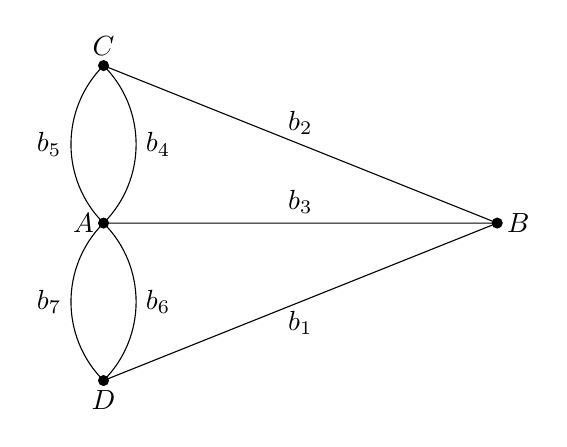
\begin{tikzpicture}
		\fill(0,0)coordinate(A)circle(2pt)node[left]{$A$}
			(5,0)coordinate(B)circle(2pt)node[right]{$B$}
			(0,2)coordinate(C)circle(2pt)node[above]{$C$}
			(0,-2)coordinate(D)circle(2pt)node[below]{$D$};
		\draw(A)--(B)node[midway,above]{$b_3$}
			(A)to[out=45,in=-45]node[midway,right]{$b_4$}(C)
			(A)to[out=135,in=-135]node[midway,left]{$b_5$}(C)
			(A)to[out=-45,in=45]node[midway,right]{$b_6$}(D)
			(A)to[out=-135,in=135]node[midway,left]{$b_7$}(D)
			(C)--(B)node[midway,above]{$b_2$}--(D)node[midway,below]{$b_1$};
	\end{tikzpicture}
	\caption{七桥问题}
	\label{figure:图论.七桥问题}
\end{figure}

如\cref{figure:图论.七桥问题} 所示,
令\begin{equation*}
	V = \{A,B,C,D\},
	\qquad
	E = \{\AutoTuple{b}{7}\},
\end{equation*}
则\((V,E)\)是一个无向图,
\(A,B,C,D\)都是这个图的顶点,
\(\AutoTuple{b}{7}\)都是这个图的边,
\(b_1\)的端点是\(B,D\),
\(b_2\)的端点是\(B,C\),
\(b_3\)的端点是\(A,B\),
\(b_4\)和\(b_5\)的端点都是\(A,C\),
\(b_6\)和\(b_7\)的端点都是\(A,D\).

\begin{example}[过河问题]
%@see: 《离散数学》(邓辉文) P169 习题6.1 6.(过河问题)
某人挑一担菜,带着一条狼和一只羊,要从河的一边到另一边.
由于渡船太小,只能带狼、羊、菜中的一样过河.
当人不在场时,狼要吃羊,羊要吃菜.
请尝试建立图模型,给出解决方法.
\begin{solution}
不妨忽略渡船在河中航行的时间,
那么只要人位于出发地,就不会位于目的地,反之亦然,狼、羊、菜同理,
可以看出人、狼、羊、菜各自所处位置可以用\(0,1\)两个数字表示,
用\(0\)表示“在出发地”,用\(1\)表示“在目的地”.
于是我们可以用4位数字,从高位到低位,依次表示人、狼、羊、菜的状态.
由题意可知,把人、狼、羊、菜看作一个整体,总的状态数是\(2^4 = 16\)种,
其中\(1100,1001,1000,0111,0110,0011\)这6种状态是非法状态,
无法避免狼吃羊或羊吃菜;
在去掉这6种非法状态以后,
合法状态就只剩下\(1111,1110,1101,1011,1010,0101,0100,0010,0001,0000\)这10种.

接下来,我们需要确定各个状态是否可以相互转化.
因为每次只能带狼、羊、菜种的一样过河,
所以每次状态转移都有代表人的数位和狼、羊、菜种某一样对应的数位发生翻转.
于是我们可以得到如下的状态图:
\begin{center}
	\tikzset{every state/.style={minimum size=1cm}}
	% requires `\usetikzlibrary{automata}'
	\begin{tikzpicture}[node distance=2cm]
		\node[state](S00){0000};
		\node[state](S10)[below of=S00]{1010};
		\node[state](S02)[right of=S10]{0010};
		\node[state](S11)[below of=S02]{1011};
		\node[state](S14)[above of=S02]{1110};
		\node[state](S04)[right of=S14]{0100};
		\node[state](S13)[below of=S04]{1101};
		\node[state](S01)[below of=S13]{0001};
		\node[state](S05)[right of=S13]{0101};
		\node[state](S15)[below of=S05]{1111};

		\draw(S00)--(S10)--(S02)--(S14)--(S04)--(S13)--(S01)--(S11)--(S02)
			(S13)--(S05)--(S15);
	\end{tikzpicture}
\end{center}

从图中可以看出,
不论是沿着\(0000,\allowbreak1010,\allowbreak0010,\allowbreak1110,\allowbreak0100,\allowbreak1101,\allowbreak0101,\allowbreak1111\)这条路径
(人羊同行,人独自返回,人狼同行,人羊返回,人菜同行,人独自返回,人羊同行),
还是沿着\(0000,\allowbreak1010,\allowbreak0010,\allowbreak1011,\allowbreak0001,\allowbreak1101,\allowbreak0101,\allowbreak1111\)这条路径
(人羊同行,人独自返回,人菜同行,人羊返回,人狼同行,人独自返回,人羊同行),
均可从初始状态\(0000\)抵达目标状态\(1111\).
\end{solution}
\end{example}

\subsection{图中元素的计数,图的分类}
\begin{definition}
%@see: 《Graph Theory》(Reinhard Diestel) P2
设图\(G = (V,E)\),
定义:\begin{gather*}
	\abs{G} \defeq \card V, \\
	\norm{G} \defeq \card E.
\end{gather*}
把\(\abs{G}\)称为“\(G\)的\DefineConcept{阶数}(order)”
或“\(G\)的\DefineConcept{顶点数}”.
把\(\norm{G}\)称为“\(G\)的\DefineConcept{边数}”.
\end{definition}

\begin{definition}
%@see: 《离散数学》(邓辉文) P166
有\(n\)个顶点的图,
称为 \DefineConcept{\(n\)阶图}.
\end{definition}

\begin{definition}
%@see: 《离散数学》(邓辉文) P166
有\(n\)个顶点、\(m\)条边(弧)的图,
称为 \DefineConcept{\((n,m)\)图}.
\end{definition}

\begin{definition}
%@see: 《离散数学》(邓辉文) P167
若图\(G = (V,E)\)
满足\(V = \emptyset\),
则称“\(G\)是\DefineConcept{空图}(empty graph)”,
记作\(\emptyset\).
\end{definition}

\begin{definition}
%@see: 《离散数学》(邓辉文) P167
若图\(G = (V,E)\)
满足\(V \neq \emptyset,E = \emptyset\),
则称“\(G\)是\DefineConcept{零图}(discrete graph)”.
特别地,\(k\)阶零图记作\(N_k\),
仅有一个顶点的零图称为\DefineConcept{平凡图}(trivial graph).
\end{definition}

\begin{definition}
%@see: 《离散数学》(邓辉文) P171 习题6.2 4.
将有向图\(G\)的有向边都换成无向边,
得到的无向图\(H\)称为“\(G\)的\DefineConcept{基础图}”.
\end{definition}

\begin{definition}
%@see: 《离散数学》(邓辉文) P167
设边\(e\)与顶点\(u,v\)关联.
如果\(u = v\),
则称“\(e\)是一条\DefineConcept{自环}(loop)”.
\end{definition}

如\cref{figure:图论.带有自环的无向图} 所示,顶点\(v_2\)有\(e_1,e_2\)两个自环.

\begin{figure}[hbt]
%@see: 《离散数学》(邓辉文) P166 图6-4(a)
%@see: 《离散数学》(邓辉文) P166 图6-9(a)
	\centering
	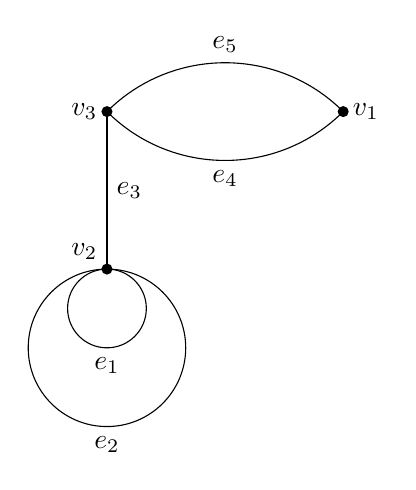
\begin{tikzpicture}
		\fill(3,2)coordinate(v1)node[right]{$v_1$}circle(2pt);
		\fill(0,0)coordinate(v2)node[above left]{$v_2$}circle(2pt);
		\fill(0,2)coordinate(v3)node[left]{$v_3$}circle(2pt);
		\draw(v2)++(0,-.5)circle(.5) (v2)++(0,-1)node[below]{$e_1$};
		\draw(v2)++(0,-1)circle(1) (v2)++(0,-2)node[below]{$e_2$};
		\draw(v2)--(v3)node[midway,right]{$e_3$};
		\draw(v1)to[out=-135,in=-45]node[midway,below]{$e_4$}(v3);
		\draw(v1)to[out=135,in=45]node[midway,above]{$e_5$}(v3);
	\end{tikzpicture}
	\caption{}
	\label{figure:图论.带有自环的无向图}
\end{figure}

\begin{definition}
%@see: 《离散数学》(邓辉文) P167
设边\(e_1\)与顶点\(u_1,v_1\)关联,
边\(e_2\)与顶点\(u_2,v_2\)关联.
如果\(u_1 = u_2,
v_1 = v_2\),
则称“\(e_1,e_2\)是一组\DefineConcept{多重边}(multiple edges)”,
或称“\(e_1,e_2\)是一组\DefineConcept{平行边}”.
\end{definition}

如\cref{figure:图论.七桥问题} 所示,
\(b_4,b_5\)是一组多重边,
\(b_6,b_7\)是另一组多重边.

\begin{definition}
%@see: 《离散数学》(邓辉文) P167
给定顶点\(u_0,v_0\),
其多重边的边数\begin{equation*}
	\card\Set{
		e \in E
		\given
		\text{$e$与$u_0,v_0$关联}
	}
\end{equation*}
称为“\(u_0\)与\(v_0\)之间的边的\DefineConcept{重数}(multiplicity)”.
\end{definition}

如\cref{figure:图论.七桥问题} 所示,
顶点\(A,C\)之间的边的重数为\(2\).

\subsection{简单图,完全图,补图}
\begin{definition}
%@see: 《离散数学》(邓辉文) P167 定义6-4
设图\(G\)既没有自环,也没有多重边,
则称“\(G\)是\DefineConcept{简单图}(simple graph)”.
\end{definition}

如\cref{figure:图论.彼得森图} 所示,
彼得森图是简单图.

\begin{definition}
%@see: 《离散数学》(邓辉文) P167 定义6-5
如果\(n\)阶简单无向图\(G\)中任意一个顶点都与其余\(n-1\)个顶点邻接,
则称“\(G\)是\(n\)阶\DefineConcept{完全无向图}(complete graph)”,
记作\(K_n\).
\end{definition}

\begin{figure}[hbt]
%@see: 《离散数学》(邓辉文) P167 图6-5
	\centering
	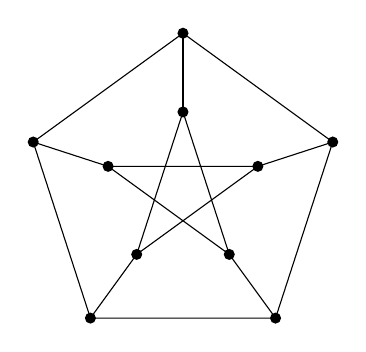
\begin{tikzpicture}
		\foreach \j in {0,...,4} {
			\fill({cos(\j*72+90)},{sin(\j*72+90)})coordinate(A\j)circle(2pt);
			\fill({2*cos(\j*72+90)},{2*sin(\j*72+90)})coordinate(B\j)circle(2pt);
			\draw(A\j)--(B\j);
		}
		\draw(A0)--(A2) (A1)--(A3) (A2)--(A4) (A3)--(A0) (A4)--(A1);
		\draw(B0)--(B1)--(B2)--(B3)--(B4)--(B0);
	\end{tikzpicture}
	\caption{彼得森图}
	\label{figure:图论.彼得森图}
\end{figure}

\begin{figure}[hbt]
%@see: 《离散数学》(邓辉文) P168 图6-6
	\centering
	\def\subwidth{.3\linewidth}
	\begin{subfigure}[b]{\subwidth}
		\centering
		\def\n{3}  % 控制顶点数
		\def\b{90}  % 控制图像绕其几何中心旋转的角度(相位)
		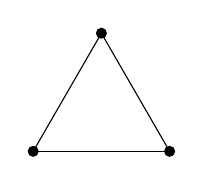
\begin{tikzpicture}
			\pgfmathsetmacro{\m}{\n-1}
			\pgfmathsetmacro{\a}{360/\n}
			\foreach \j in {0,...,\m} {
				\fill({cos(\j*\a+\b)},{sin(\j*\a+\b)})coordinate(A\j)circle(2pt);
			}
			\foreach \j in {0,...,\m} {
				\foreach \k in {0,...,\m} {
					\ifnum\j<\k\relax
						\draw(A\j)--(A\k);
					\fi
				}
			}
		\end{tikzpicture}
		\caption{\n 阶完全无向图\(K_\n\)}
	\end{subfigure}~\begin{subfigure}[b]{\subwidth}
		\centering
		\def\n{4}
		\def\b{45}
		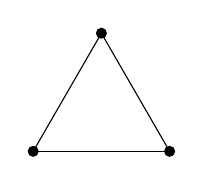
\begin{tikzpicture}
			\pgfmathsetmacro{\m}{\n-1}
			\pgfmathsetmacro{\a}{360/\n}
			\foreach \j in {0,...,\m} {
				\fill({cos(\j*\a+\b)},{sin(\j*\a+\b)})coordinate(A\j)circle(2pt);
			}
			\foreach \j in {0,...,\m} {
				\foreach \k in {0,...,\m} {
					\ifnum\j<\k\relax
						\draw(A\j)--(A\k);
					\fi
				}
			}
		\end{tikzpicture}
		\caption{\n 阶完全无向图\(K_\n\)}
	\end{subfigure}~\begin{subfigure}[b]{\subwidth}
		\centering
		\def\n{5}
		\def\b{90}
		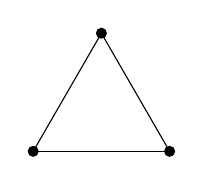
\begin{tikzpicture}
			\pgfmathsetmacro{\m}{\n-1}
			\pgfmathsetmacro{\a}{360/\n}
			\foreach \j in {0,...,\m} {
				\fill({cos(\j*\a+\b)},{sin(\j*\a+\b)})coordinate(A\j)circle(2pt);
			}
			\foreach \j in {0,...,\m} {
				\foreach \k in {0,...,\m} {
					\ifnum\j<\k\relax
						\draw(A\j)--(A\k);
					\fi
				}
			}
		\end{tikzpicture}
		\caption{\n 阶完全无向图\(K_\n\)}
	\end{subfigure}
	\caption{完全图}
\end{figure}

\begin{proposition}
\(n\)阶完全无向图\(K_n\)的边数为
\(n(n-1)/2\).
\end{proposition}

\begin{definition}
设\(G\)是\(n\)阶简单有向图.
若\(G\)中任意顶点都与其余\(n-1\)个顶点邻接,
则称“\(G\)是\(n\)阶\DefineConcept{完全有向图}”.
\end{definition}

我们将完全无向图、完全有向图统称为\DefineConcept{完全图}.

\begin{definition}
%@see: 《离散数学》(邓辉文) P171 习题6.2 4.
基础图是完全图的有向图,称为\DefineConcept{竞赛图}.
% 另一种表述方式:
% 将\(n\)阶完全无向图\(K_n\)的边
% 任意加一个方向所得到的有向图
% 称为\(n\)阶\DefineConcept{竞赛图}.
\end{definition}


\begin{definition}
%@see: 《离散数学》(邓辉文) P168 定义6-6
设\(G\)是\(n\)阶简单无向图.
由\(G\)的所有顶点
以及能使\(G\)成为\(K_n\)需要添加的边构成的图,
称为“\(G\)的\DefineConcept{补图}(complementary graph)”,
记为\(\overline{G}\).
\end{definition}

\begin{figure}[hbt]
%@see: 《离散数学》(邓辉文) P168 图6-6
%@see: 《离散数学》(邓辉文) P173 图6-16
	\centering
	\def\subwidth{.3\linewidth}
	\begin{subfigure}[b]{\subwidth}
		\centering
		\def\n{5}
		\def\b{90}
		\begin{tikzpicture}
			\pgfmathsetmacro{\m}{\n-1}
			\pgfmathsetmacro{\a}{360/\n}
			\foreach \j in {0,...,\m} {
				\fill({cos(\j*\a+\b)},{sin(\j*\a+\b)})coordinate(A\j)circle(2pt);
				\draw({cos(\j*\a+\b)},{sin(\j*\a+\b)})
					--({cos((\j+1)*\a+\b)},{sin((\j+1)*\a+\b)});
			}
			\draw(A0)node[above]{1}
				(A1)node[left]{2}
				(A2)node[left]{3}
				(A3)node[right]{4}
				(A4)node[right]{5};
		\end{tikzpicture}
		\caption{}
		\label{figure:图论.补图.原图1}
	\end{subfigure}~\begin{subfigure}[b]{\subwidth}
		\centering
		\def\n{5}
		\def\b{90}
		\begin{tikzpicture}
			\pgfmathsetmacro{\m}{\n-1}
			\pgfmathsetmacro{\a}{360/\n}
			\foreach \j in {0,...,\m} {
				\fill({cos(\j*\a+\b)},{sin(\j*\a+\b)})coordinate(A\j)circle(2pt);
				\draw({cos(\j*\a+\b)},{sin(\j*\a+\b)})
					--({cos((\j+2)*\a+\b)},{sin((\j+2)*\a+\b)});
			}
			\draw(A0)node[above]{1}
				(A1)node[left]{2}
				(A2)node[left]{3}
				(A3)node[right]{4}
				(A4)node[right]{5};
		\end{tikzpicture}
		\caption{}
		\label{figure:图论.补图.补图1}
	\end{subfigure}
	\caption{}
\end{figure}

\cref{figure:图论.补图.原图1} 中的图
与\cref{figure:图论.补图.补图1} 中的图
互为补图.

\begin{proposition}
%@see: 《离散数学》(邓辉文) P168
对于任意顶点\(u,v\),
若\(u\)和\(v\)在\(G\)中不邻接,
则\(u\)和\(v\)在\(\overline{G}\)中邻接;
若\(u\)和\(v\)在\(G\)中邻接,
则\(u\)和\(v\)在\(\overline{G}\)中不邻接.
\end{proposition}

\begin{example}
%@see: 《离散数学》(邓辉文) P169 习题6.1 9.
设\(n\)阶简单无向图\(G\)有\(m\)条边,
求\(G\)的补图\(\overline{G}\)的边数.
\begin{solution}
因为\(n\)阶完全图的边数是\(\frac{n(n-1)}2\),
所以\(G\)的补图\(\overline{G}\)的边数为\(\frac{n(n-1)}2-m\).
\end{solution}
\end{example}

\section{顶点的度数}
\begin{definition}
%@see: 《离散数学》(邓辉文) P169 定义6-7
设\(G = (V,E)\)是无向图,\(v \in V\),
把与顶点\(v\)关联的所有边的边数
称为“顶点\(v\)的\DefineConcept{度数}(degree)”,
记为\(\deg v\).
\end{definition}

在\cref{figure:图论.七桥问题} 中,
\(A\)的度数为5,
\(B,C,D\)的度数均为3.

如\cref{figure:图论.带有自环的无向图} 所示,
\(v_1\)的度数为2,
\(v_2\)的度数为5,
\(v_3\)的度数为3.
特别要注意\(v_2\),
它关联的两条自环\(e_1,e_2\),
每一条计入的度数都是2.

\begin{definition}
%@see: 《离散数学》(邓辉文) P169 定义6-8
设\(G = (V,E)\)是有向图,\(v \in V\),
把以\(v\)为起点的边的数目
称为“顶点\(v\)的\DefineConcept{出度}(out-degree)”,
记为\(\degIn v\);
把以\(v\)为终点的边的数目
称为“顶点\(v\)的\DefineConcept{入度}(in-degree)”,
记为\(\degEx v\);
把顶点\(v\)的出度与入度之和
称为“顶点\(v\)的\DefineConcept{度数}(degree)”,
记为\(\deg v\).
\end{definition}

\begin{theorem}\label{theorem:图论.握手定理}
%@see: 《离散数学》(邓辉文) P169 定理6-1(握手定理)
在任何\((n,m)\)图\(G = (V,E)\)中,
其所有顶点度数之和等于边数\(m\)的2倍,
即\[
	\sum_{v \in V} \deg v = 2m.
\]
%TODO proof
\end{theorem}

\begin{corollary}\label{theorem:图论.握手定理.推论}
%@see: 《离散数学》(邓辉文) P170 推论
在任意图中,度数为奇数的顶点个数必定为偶数.
%TODO proof
\end{corollary}

\begin{theorem}
%@see: 《离散数学》(邓辉文) P170 定理6-2
在任意有向图中,所有顶点的出度之和等于入度之和.
\begin{proof}
设\(G = (V,E)\)是\(n\)阶竞赛图,
则其边数为\(\abs{E} = \frac{n(n-1)}2\),
并且,对于任意\(v \in V\),有\[
	\degEx v + \degIn v = n-1.
\]
于是,根据竞赛图的定义可知\[
	\sum_{v \in V} \degEx v
	= \sum_{v \in V} \degIn v
	= \abs{E}.
	\qedhere
\]
\end{proof}
\end{theorem}

\begin{example}
%@see: 《离散数学》(邓辉文) P171 习题6.2 4.
证明:任意一个竞赛图的所有顶点的出度的平方和等于其入度的平方和.
%TODO proof
\end{example}

\begin{example}
%@see: 《离散数学》(邓辉文) P171 习题6.2 2.
无向图\(G\)有6条边,有1个3度顶点、1个5度顶点,剩余的顶点均为2度,求\(G\)的阶数.
\begin{solution}
设2度顶点的个数为\(n_2\),
则由\cref{theorem:图论.握手定理} 可知
\(3 + 5 + 2 n_2 = 12\),
解得\(n_2 = 2\),
于是\(G\)的阶数为\(1 + 1 + n_2 = 4\).
\end{solution}
\end{example}

\begin{definition}
%@see: 《离散数学》(邓辉文) P170
在任意图\(G = (V,E)\)中,
度数为0的顶点
称为\DefineConcept{孤立点}(isolated vertex),
度数为1的顶点
称为\DefineConcept{悬挂点}(pendant vertex).
\end{definition}

\begin{definition}
%@see: 《离散数学》(邓辉文) P170
若简单无向图\(G\)的每个顶点的度数均为\(k\),
则称“\(G\)是一个 \DefineConcept{\(k\)-正则图}(\(k\)-regular graph)”.
\end{definition}

\begin{example}
%@see: 《离散数学》(邓辉文) P170 例6-2
设无向图\(G\)是一个\(3\)-正则\((n,m)\)图,
且\(2n-3=m\).
求\(n,m\).
\begin{solution}
由\cref{theorem:图论.握手定理} 有
\(3n = 2m\).
与\(2n-3=m\)联立方程组,
截得\(n=6,m=9\).
图\(G\)如\cref{figure:图论.正则图1} 所示.
\begin{figure}[hbt]
%@see: 《离散数学》(邓辉文) P173 图6-17(a)
	\centering
	\def\n{3}  % 控制顶点数
	\def\b{90}  % 控制图像绕其几何中心旋转的角度(相位)
	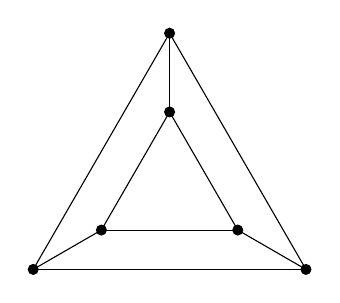
\begin{tikzpicture}
		\pgfmathsetmacro{\m}{\n-1}
		\pgfmathsetmacro{\a}{360/\n}
		\foreach \j in {0,...,\m} {
			\fill({cos(\j*\a+\b)},{sin(\j*\a+\b)})coordinate(A\j)circle(2pt);
			\fill({2*cos(\j*\a+\b)},{2*sin(\j*\a+\b)})coordinate(B\j)circle(2pt);
			\draw(A\j)--(B\j);
		}
		\foreach \j in {0,...,\m} {
			\foreach \k in {0,...,\m} {
				\ifnum\j<\k\relax
					\draw(A\j)--(A\k);
					\draw(B\j)--(B\k);
				\fi
			}
		}
	\end{tikzpicture}
	\caption{$3$-正则$(6,9)$图}
	\label{figure:图论.正则图1}
\end{figure}
\end{solution}
\end{example}

\begin{example}
%@see: 《离散数学》(邓辉文) P171 习题6.2 3.(1)
证明:\(3\)-正则图的阶数必定是偶数.
\begin{proof}
设\(G\)是\(3\)-正则\((n,m)\)图.
根据\cref{theorem:图论.握手定理} 有
\(3 n = 2 m\).
由于\(2 \mid 2 m\),
因此\(2 \mid n\),
即\(n\)必定是偶数.
\end{proof}
\end{example}

\begin{definition}
%@see: 《离散数学》(邓辉文) P170 定义6-9
在任意图\(G = (V,E)\)中,
把\[
	\Delta(G)
	\defeq
	\max_{v \in V} \deg v
\]称为\(G\)的\DefineConcept{最大度},
把\[
	\delta(G)
	\defeq
	\min_{v \in V} \deg v
\]称为\(G\)的\DefineConcept{最小度}.
\end{definition}

在\cref{figure:图论.带有自环的无向图} 中,
\(\Delta(G) = 5,
\delta(G) = 2\).

\begin{proposition}
%@see: 《离散数学》(邓辉文) P171 习题6.2 5.
设\(G\)是\((n,m)\)无向图,
则\[
	\delta(G)
	\leq
	\frac{2m}{n}
	\leq
	\Delta(G).
\]
%TODO proof
\end{proposition}

\begin{proposition}
%@see: 《离散数学》(邓辉文) P171
正则图的最大度\(\Delta(G)\)与最小度\(\delta(G)\)相等.
\end{proposition}

\begin{example}
%@see: 《离散数学》(邓辉文) P171 习题6.2 1.
证明:对于任意\(n\)阶简单图\(G\),
有\(\Delta(G) \leq n-1\).
%TODO proof
\end{example}

\begin{example}
%@see: 《离散数学》(邓辉文) P171 习题6.2 8.
设无向图\(G\)有10条边,
3度和4度顶点各2个,
其余顶点的度数均小于3.
求\(G\)至少有多少个顶点?
在最少顶点的情况下,
求\(G\)的度数序列、最大度\(\Delta(G)\)和最小度\(\delta(G)\).
%TODO \(G\)至少有7个顶点,度数序列是\(4,4,3,3,2,2,2\),最大度\(\Delta(G) = 4\),最小度\(\delta(G) = 2\)
\end{example}

\begin{definition}
%@see: 《离散数学》(邓辉文) P170 定义6-9
在有向图\(G = (V,E)\)中,
把\[
	\Delta^+(G)
	\defeq
	\max_{v \in V} \degEx v
\]称为\(G\)的\DefineConcept{最大出度},
把\[
	\delta^+(G)
	\defeq
	\min_{v \in V} \degEx v
\]称为\(G\)的\DefineConcept{最小出度},
把\[
	\Delta^-(G)
	\defeq
	\max_{v \in V} \degIn v
\]称为\(G\)的\DefineConcept{最大入度},
把\[
	\delta^-(G)
	\defeq
	\min_{v \in V} \degIn v
\]称为\(G\)的\DefineConcept{最小入度}.
\end{definition}

\begin{definition}
%@see: 《离散数学》(邓辉文) P171
对于无向图\(G = (V,E)\),
\(V = \{\AutoTuple{v}{n}\}\),
把\[
	\deg v_1,\dotsc,\deg v_n
\]
称为“\(G\)的\DefineConcept{度数序列}”.
\end{definition}

在\cref{figure:图论.带有自环的无向图} 中,
图的度数序列为\(2,5,3\).

\begin{example}
%@see: 《离散数学》(邓辉文) P171 例6-3
试讨论:是否存在一个无向图,其度数序列分别为
\(7,5,4,2,2,1\)?
\begin{solution}
由于上述度数序列中,
奇数的个数为奇数,
于是由\cref{theorem:图论.握手定理.推论} 可知,
不存在满足条件的图.
\end{solution}
\end{example}

%TODO 思考:对于给定的自然数序列\(\AutoTuple{d}{n}\),存在一个无向图(及简单无向图),其度数序列为\(\AutoTuple{d}{n}\)的充分必要条件是什么?
\begin{example}
%@see: 《离散数学》(邓辉文) P171 习题6.2 9.
证明:对于给定的自然数序列\(\AutoTuple{d}{n}\),
存在一个无向图\(G\),
其度数序列为\(\AutoTuple{d}{n}\)的充分必要条件是\[
	\sum_{i=1}^n d_i \equiv 0\pmod2.
\]
%TODO proof
\end{example}

\section{子图,图的运算,图同构}
\subsection{子图}
\begin{definition}
%@see: 《离散数学》(邓辉文) P171 定义6-10
设\(G = (V,E)\)和\(H = (W,F)\)都是图.
若\(W \subseteq V\)且\(F \subseteq E\),
则称“\(H\)是\(G\)的一个\DefineConcept{子图}(subgraph)”
%@see: 《Graph Theory》(Reinhard Diestel) P3
“\(G\)是\(H\)的一个\DefineConcept{超图}(supergraph)”,
记作\(H \subseteq G\).
\end{definition}

\begin{definition}
%@see: 《Graph Theory》(Reinhard Diestel) P3
设图\(H \subseteq G\)且\(H \neq G\),
则称“\(H\)是\(G\)的一个\DefineConcept{真子图}(\(H\) is a \emph{proper subgraph} of \(G\))”,
记作\(H \subset G\).
\end{definition}

\begin{definition}
%@see: 《离散数学》(邓辉文) P172 定义6-10
设\(H = (W,F)\)是\(G = (V,E)\)的子图.
如果\(W = V\),
则称“\(H\)是\(G\)的一个\DefineConcept{生成子图}(spanning subgraph)”.
\end{definition}

%@see: 《离散数学》(邓辉文) P172
常见的4种产生\(G = (V,E)\)的子图的方式:
\begin{center}
\begin{tblr}{p{2cm}p{13cm}}
	{\(G[W]\)法} &
	设\(W \subseteq V\).
	以\(W\)为顶点集,
	以两端点均属于\(W\)的所有边为边集,
	构成的子图,
	称为\DefineConcept{由\(W\)导出的子图}(induced subgraph by \(W\)),
	记作\(G[W]\).
	\\
	{\(G-W\)法} &
	设\(W \subseteq V\).
	将由\(V-W\)导出的子图\(G[V-W]\)
	记作\(G-W\).
	\\
	{\(G[F]\)法} &
	设\(F \subseteq E\).
	以\(F\)为边集,
	以\(F\)中边的所有端点为顶点集,
	构成的子图,
	称为\DefineConcept{由\(F\)导出的子图}(induced subgraph by \(F\)),
	记作\(G[F]\).
	\\
	{\(G-F\)法} &
	设\(F \subseteq E\).
	将由\(E-F\)导出的子图\(G[E-F]\)
	记作\(G-F\).
	\\
\end{tblr}
\end{center}

\begin{proposition}
%@see: 《离散数学》(邓辉文) P172
设\(G = (V,E)\)是\(n\)阶简单无向图,
则\(G\)的补图为\(\overline{G} = K_n - E\).
\end{proposition}

我们除了可以产生子图以外,还可以反过来,在图\(G = (V,E)\)的基础上,
通过在\(V\)中某些顶点之间增加一些新的边\(U\),得到一个更大的图\(G + U\).

\subsection{图的运算}
图的运算就是通过一些操作,产生新的图.
上一小节讨论的子图的产生方法,在本质上是图的一种运算,但它只涉及一个图.
本章第一节讨论的补图的计算方法,同样在本质上是图的一种运算,而且它涉及两个图.

下面我们来讨论两个图之间的运算.
\begin{definition}
%@see: 《离散数学》(邓辉文) P173 定义6-11
设\(G_1 = (V_1,E_1)\)和\(G_2 = (V_2,E_2)\)都是无向图(或有向图).
\begin{itemize}
	\item 把满足\[
		E = E_1 \cup E_2,
		\qquad
		V = V_1 \cup V_2
	\]的图\(G = (V,E)\)
	称为“\(G_1\)与\(G_2\)的\DefineConcept{并}”,
	记作\(G_1 \cup G_2\).

	\item 把满足\[
		E = E_1 \cap E_2,
		\qquad
		V = V_1 \cap V_2
	\]的图\(G = (V,E)\)
	称为“\(G_1\)与\(G_2\)的\DefineConcept{交}”,
	记作\(G_1 \cap G_2\).

	\item 把满足\[
		E = E_1 - E_2,
		\qquad
		V = V_1
	\]的图\(G = (V,E)\)
	称为“\(G_1\)与\(G_2\)的\DefineConcept{差}”,
	记作\(G_1 - G_2\).

	\item 把满足\[
		E = E_1 \symdiff E_2,
		\qquad
		V = V_1 \cup V_2
	\]的图\(G = (V,E)\)
	称为“\(G_1\)与\(G_2\)的\DefineConcept{对称差}”
	或“\(G_1\)与\(G_2\)的\DefineConcept{环和}(ring sum)”,
	记作\(G_1 \symdiff G_2\).
\end{itemize}
\end{definition}

\subsection{图同构}
由于图的拓扑不变性,
两个看上去不同的图,有可能本质上是同一个图,
这就是图同构的问题.

\begin{definition}
%@see: 《离散数学》(邓辉文) P173 定义6-12
%@see: 《Graph Theory》(Reinhard Diestel) P3
设\(G_1 = (V_1,E_1)\)和\(G_2 = (V_2,E_2)\)都是无向图(或有向图).
如果存在双射\(\rho,\sigma\)满足\begin{equation*}
	(\forall u_1,v_1 \in V_1)
	(\forall e_1 \in E_1)
	\left[
		\text{$e_1$与$u_1,v_1$是关联的}
		\iff
		\text{$\sigma(v_1)$与$\rho(u_1),\rho(v_1)$是关联的}
	\right],
\end{equation*}
则称“图\(G_1\)与\(G_2\) \DefineConcept{同构}%
(\(G_1\) and \(G_2\) are \emph{isomorphic})”,
记作\(G_1 \Isomorphism G_2\).
\end{definition}

由定义可知,两个图同构,当且仅当这两个图的顶点与边分别一一对应,并且保持顶点与边的关联关系.
或者更直观地说,两个图同构,是指其中一个图仅经过顶点的位移和边的形变这两种变换,就可以变为另一个图.

容易看出,
\cref{figure:图论.补图.原图1,figure:图论.补图.补图1} 中的两个图是同构的,
\cref{figure:图论.正则图1,figure:图论.K33} 中的两个图是不同构的.

\begin{figure}[hbt]
%@see: 《离散数学》(邓辉文) P173 图6-17(b)
	\centering
	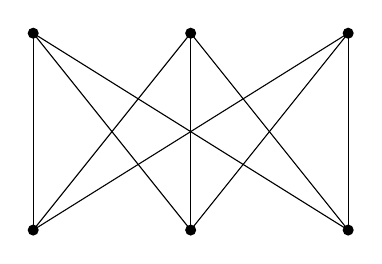
\begin{tikzpicture}
		\fill(0,0)coordinate(A1)circle(2pt);
		\fill(2,0)coordinate(A2)circle(2pt);
		\fill(4,0)coordinate(A3)circle(2pt);
		\fill(0,2.5)coordinate(B1)circle(2pt);
		\fill(2,2.5)coordinate(B2)circle(2pt);
		\fill(4,2.5)coordinate(B3)circle(2pt);
		\foreach \j in {1,...,3} {
			\foreach \k in {1,...,3} {
				\draw(A\j)--(B\k);
			}
		}
	\end{tikzpicture}
	\caption{}
	\label{figure:图论.K33}
\end{figure}

在判断两个有向图是否同构时,要特别注意边的方向的一致性.

\begin{definition}
%@see: 《离散数学》(邓辉文) P175 习题6.3 7.
若一个简单无向图\(G\)与它的补图\(\overline{G}\)同构,
则称“\(G\)是一个\DefineConcept{自补图}”.
\end{definition}

\begin{example}
%@see: 《离散数学》(邓辉文) P175 习题6.3 7.(2)
设\(G\)是\(n\)阶自补图.
证明:\(K_n\)的边数是偶数.
%TODO proof
\end{example}

\begin{example}
%@see: 《离散数学》(邓辉文) P175 习题6.3 7.(3)
设\(G\)是\(n\ (n\geq2)\)阶自补图.
证明:存在正整数\(k\)使得\(n=4k\)或\(n=4k+1\).
%TODO proof
\end{example}

2015年,芝加哥大学 Babai 教授给出了在拟多项式时间复杂度内判定两个图同构的算法.
%TODO 看一下参考文献

\begin{conjecture}[乌拉姆猜想(1929)]
%@see: 《离散数学》(邓辉文) P174 乌拉姆(Ulam)猜想(1929)
设\(G_1,G_2\)都是简单无向图,
\(V(G_1) = \{\AutoTuple{v}{n}\},
V(G_2) = \{\AutoTuple{w}{n}\}\).
若对于任意\(i=1,2,\dotsc,n\)均有\(G_1 - v_i \Isomorphism G_2 - w_i\),
则\(G_1 \Isomorphism G_2\).
%@see: https://mathworld.wolfram.com/UlamsConjecture.html
\end{conjecture}

\section{路,回路}
在途中,经常需要考虑从一个顶点出发,沿着一些边连续移动到另一个顶点的问题.
这就是路的概念,它与七桥问题密切相关.

\subsection{路}
\begin{definition}
%@see: 《离散数学》(邓辉文) P175 定义6-13
在任意一个图\(G = (V,E)\)中,
将顶点、边交替出现的序列\[
	L: v_0 e_1 v_1 e_2 v_2 \dotso v_{i-1} e_i v_i \dotso e_l v_l
\]称为“从\(v_0\)到\(v_l\)的一条\DefineConcept{路}(walk,way)”,
将\(v_0\)称为“路\(L\)的\DefineConcept{起点}”,
将\(v_l\)称为“路\(L\)的\DefineConcept{终点}”,
将\(L\)所经过的边数\(l\)称为\DefineConcept{路长}(length of walk)或\DefineConcept{跳数}(hop number).
特别地,只有一个顶点、路长为\(0\)的序列,称为\DefineConcept{平凡路}.
\end{definition}

在不引起混淆的情况下,可以将路\(L: v_0 e_1 v_1 e_2 v_2 \dotso v_{i-1} e_i v_i \dotso e_l v_l\)
简记为\[
	L: v_0 v_1 v_2 \dotso v_{i-1} v_i \dotso v_l
\]
或\[
	L: e_1 e_2 \dotso e_i \dotso e_l.
\]

\begin{definition}
%@see: 《离散数学》(邓辉文) P175
顶点不重复的路,称为\DefineConcept{路径}(path).
\end{definition}

\begin{definition}
%@see: 《离散数学》(邓辉文) P175
边不重复的路,称为\DefineConcept{轨迹}(trail).
\end{definition}

\begin{proposition}
%@see: 《离散数学》(邓辉文) P175
路径一定是轨迹,轨迹不一定是路径.
%TODO proof
\end{proposition}

\begin{definition}
%@see: 《离散数学》(邓辉文) P175 定义6-14
在图\(G = (V,E)\)中,
把从顶点\(u\)到顶点\(v\)、边数最少的路的路长
称为“\(u\)到\(v\)的\DefineConcept{距离}(distance)”,
记作\(d(u,v)\).
当从\(u\)到\(v\)的路不存在时,
记\(d(u,v) = \infty\).
\end{definition}

显然,对于任意顶点\(u,v \in V\)有\(d(u,v) \geq 0\).

\begin{definition}
%@see: 《离散数学》(邓辉文) P175 定义6-14
设图\(G = (V,E)\).
把\[
	\max_{u,v \in V} d(u,v)
\]称为“图\(G\)的\DefineConcept{直径}(diameter)”,
记作\(\diam G\).
\end{definition}

\subsection{回路}
\begin{definition}
%@see: 《离散数学》(邓辉文) P176 定义6-15
起点与终点相同的路,称为\DefineConcept{回路}(circuit).
\end{definition}

\begin{definition}
%@see: 《离散数学》(邓辉文) P176 定义6-15
边不重复的回路,称为\DefineConcept{简单回路}(simple circuit)或\DefineConcept{闭迹}(closed trail).
\end{definition}

\begin{definition}
%@see: 《离散数学》(邓辉文) P176 定义6-15
除了起点、终点重合以外,其余顶点各个不同的简单回路,
称为\DefineConcept{圈}或\DefineConcept{环}(cycle).
\end{definition}
\begin{remark}
注意区分“环”与“自环”这两个概念:
自环是边,环是路.
\end{remark}

由于回路的路长至少是1,
所以平凡路不是回路.

\begin{example}
举例说明:简单回路不一定是圈.
%TODO
\end{example}

\begin{definition}
%@see: 《离散数学》(邓辉文) P176
有\(n\)个顶点的圈,称为 \DefineConcept{\(n\)阶圈},记作\(C_n\).
\end{definition}

\begin{definition}
%@see: 《离散数学》(邓辉文) P176
给\(n-1\)阶圈\(C_{n-1}\)增加一个顶点\(u\),
再使\(u\)与\(C_{n-1}\)的每个顶点邻接,
得到的图称为 \DefineConcept{\(n\)阶轮图},记作\(W_n\).
\end{definition}

\begin{theorem}
%@see: 《离散数学》(邓辉文) P176 定理6-3
在无向图\(G = (V,E)\)中,
若任意\(v \in V\)有\(\deg v \geq 2\),
则\(G\)中存在圈.
%TODO proof
\end{theorem}

\begin{example}
%@see: 《离散数学》(邓辉文) P177 习题6.4 5.
设无向图\(G\)的任意两个顶点之间都存在一条路.
证明:\(G\)的任意两条最长轨迹存在公共顶点.
%TODO proof
\end{example}

\begin{example}
%@see: 《离散数学》(邓辉文) P177 习题6.4 6.
设\(G\)是简单有向图,记\(k = \max\{\degEx G,\degIn G\}\).
证明:\(G\)中存在路长至少为\(k\)的轨迹.
%TODO proof
\end{example}

\begin{example}
%@see: 《离散数学》(邓辉文) P177 习题6.4 7.
证明:在一个没有回路的竞赛图\(G\)中,对于任意顶点\(u,v\),总有\(\degEx u \neq \degEx v\).
%TODO proof
\end{example}

\begin{example}
%@see: 《离散数学》(邓辉文) P177 习题6.4 8.
设有向图\(G = (V,E)\)满足\((\forall v \in V)[\degIn v \geq 2]\).
证明:\(G\)中至少含有两个不同的圈.
%TODO proof
\end{example}

\subsection{杜克路}
%@see: https://doc.sagemath.org/html/en/reference/combinat/sage/combinat/path_tableaux/dyck_path.html
%@see: https://mathweb.ucsd.edu/~duqiu/files/Nankai18.pdf
%@see: https://users.monash.edu/~heikod/cpg2020/CPGparts1and2.pdf
%@see: https://pages.stat.wisc.edu/~callan/papers/polygon_dissections/polygon_dissections.pdf
\begin{definition}
%@see: 《组合数学及其应用》(曾光) P87 定义2.28(格路径)
在二维平面\(\mathbb{Z}^2\)沿整数格点按一定步法行走的路径称为\DefineConcept{格路径},
把相邻两个格点之间的线段称为格路径的\DefineConcept{步},
所走的步数称为格路径的\DefineConcept{长度}.
\end{definition}
\begin{definition}
%@see: 《组合数学及其应用》(曾光) P87 定义2.29(Dyck路)
长为\(2n\)的\DefineConcept{杜克路}(Dyck path)
%@see: https://mathworld.wolfram.com/DyckPath.html
是指只用“上步”\((1,1)\)和“下步”\((1,-1)\),
从\((0,0)\)到\((2n,0)\)的
不允许走到\(x\)轴下方的格路径,
把\(n\)称为杜克路的\DefineConcept{阶}.
\end{definition}
\begin{definition}
把\begin{equation*}
	\frac{(2n)!}{(n+1)! \cdot n!}
	\quad(n=1,2,\dotsc)
\end{equation*}
称为“第\(n\)个\DefineConcept{卡塔兰数}(Catalan number)”,
记作\(C_n\).
%@see: https://mathworld.wolfram.com/CatalanNumber.html
\end{definition}
\begin{table}[htb]
	\centering
	\begin{tblr}{c|*9c}
		\hline
		\(n\) & \(1\) & \(2\) & \(3\) & \(4\) & \(5\) & \(6\) & \(7\) & \(8\) & \(9\) \\
		\hline
		\(C_n\) & \(1\) & \(2\) & \(5\) & \(14\) & \(42\) & \(132\)
		& \(429\) & \(1430\) & \(4862\) \\
		\hline
	\end{tblr}
	\caption{前9个卡塔兰数}
%@Mathematica: Table[CatalanNumber[n], {n, 1, 10}]
\end{table}
\begin{theorem}
%@see: 《组合数学及其应用》(曾光) P88 定理2.26
全体\(n\)阶杜克路的基数等于第\(n\)个卡塔兰数.
\end{theorem}

\section{图的连通性}
\begin{definition}
%@see: 《离散数学》(邓辉文) P177 定义6-16
设图\(G = (V,E)\).
若从顶点\(u\)到\(v\)之间存在一条路,
则称“\(u\) \DefineConcept{可达} \(v\)”.
\end{definition}

由于任意一个顶点\(v\)到它自己之间总存在一条平凡路,
因此每一个顶点均可达它自己.

\begin{definition}
设图\(G = (V,E)\).
若\(u\)可达\(v\),且\(v\)可达\(u\),
则称“\(u\)和\(v\) \DefineConcept{相互可达}”.
\end{definition}

\subsection{无向图的连通性}
\begin{definition}
%@see: 《离散数学》(邓辉文) P177 定义6-17
设无向图\(G = (V,E)\).
如果对于任意两个顶点\(u,v \in V\),
\(u\)可达\(v\),
则称“\(G\)是一个\DefineConcept{连通图}(connected graph)”.
\end{definition}

\begin{definition}
%@see: 《离散数学》(邓辉文) P178 定义6-18
无向图\(G\)中极大的连通子图
称为“\(G\)的一个\DefineConcept{连通分量}(connected component)”.
\end{definition}

\begin{definition}
%@see: 《离散数学》(邓辉文) P178 定义6-18
无向图\(G = (V,E)\)的连通分量个数记为\(w(G)\).
\end{definition}

\begin{theorem}
%@see: 《离散数学》(邓辉文) P178 定理6-4
设无向图\(G = (V,E)\),
则\[
	\text{$G$是连通图}
	\iff
	w(G) = 1.
\]
\end{theorem}

\begin{corollary}
%@see: 《离散数学》(邓辉文) P178
设无向图\(G = (V,E)\),
则\[
	\text{$G$是非连通图}
	\iff
	w(G) \geq 2.
\]
\end{corollary}

\begin{example}
%@see: 《离散数学》(邓辉文) P178 例6-5
设\(G = (V,E)\)是简单无向图.
若\(G\)不是连通图,
则\(G\)的补图\(\overline{G}\)是连通图.
%TODO proof
\end{example}

\begin{example}
%@see: 《离散数学》(邓辉文) P178 例6-6
设\(G = (V,E)\)是\(n\)阶简单无向图.
证明:若\[
	(\forall u,v \in V)
	\left[
		\text{$u,v$不邻接}
		\implies
		\deg u + \deg v \geq n - 1
	\right],
\]
则\(G\)是连通图.
%TODO proof
\end{example}

\begin{theorem}
%@see: 《离散数学》(邓辉文) P178 定理6-5
设\(G = (V,E)\)是连通无向图,则\begin{itemize}
	\item 去掉\(G\)中任意简单回路\(C\)上的一条边\(e\)得到的图\(G - e\)还是连通图;
	\item 去掉一个度数为1的顶点\(v\)得到的图\(G - v\)还是连通图.
\end{itemize}
%TODO proof
\end{theorem}

\subsection{连通无向图的点连通度}
不同的连通无向图的连通的“程度”是各不相同的,有的图的连通性很“脆弱”,有的则与之相反.

\begin{definition}
%@see: 《离散数学》(邓辉文) P178 定义6-19
设\(G = (V,E)\)是连通无向图,且\(W \subset V\).
若\begin{itemize}
	\item 从\(G\)中删除\(W\)的所有顶点所得到的子图\(G-W\)不是连通图,或者\(G-W\)是1阶图,
	\item 而且删除\(W\)的任意一个真子集所得到的子图都还是连通图,
\end{itemize}
则称“\(W\)是\(G\)的\DefineConcept{点割集}(cut-set of vertices)”.

特别地,如果\(G\)的点割集是一个单元素集\(W = \{v\}\),
则称“\(v\)是\(G\)的\DefineConcept{割点}(cut point)”
或“\(v\)是\(G\)的\DefineConcept{关节点}(articulation point)”.
\end{definition}

由定义可知,1阶图的点割集为\(\emptyset\).
在\cref{figure:图论.点割集1} 中,图的点割集是\(\{a,b\},\{c,d\}\).

\begin{figure}[hbt]
%@see: 《离散数学》(邓辉文) P179 图6-27(a)
	\centering
	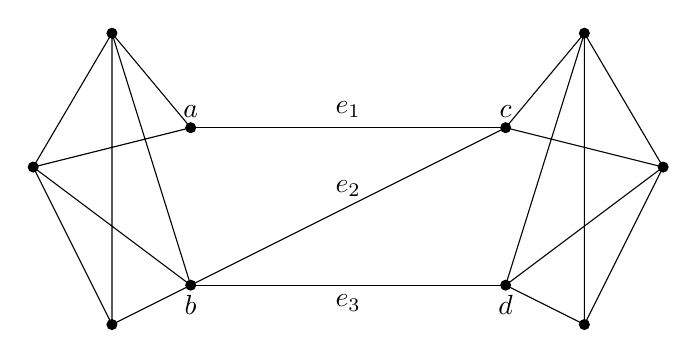
\begin{tikzpicture}
		\fill(0,0)coordinate(a)node[above]{$a$}circle(2pt);
		\fill(0,-2)coordinate(b)node[below]{$b$}circle(2pt);
		\fill(4,0)coordinate(c)node[above]{$c$}circle(2pt);
		\fill(4,-2)coordinate(d)node[below]{$d$}circle(2pt);
		\fill(-1,1.2)coordinate(v1)circle(2pt);
		\fill(-2,-.5)coordinate(v2)circle(2pt);
		\fill(-1,-2.5)coordinate(v3)circle(2pt);
		\fill(5,1.2)coordinate(u1)circle(2pt);
		\fill(6,-.5)coordinate(u2)circle(2pt);
		\fill(5,-2.5)coordinate(u3)circle(2pt);
		\draw(a)--(c)node[midway,above]{$e_1$};
		\draw(b)--(c)node[midway,above]{$e_2$};
		\draw(b)--(d)node[midway,below]{$e_3$};
		\draw(v1)--(a) (v1)--(v2) (v1)--(v3) (v1)--(b) (v2)--(a) (v2)--(b) (v2)--(v3) (v3)--(b);
		\draw(u1)--(c) (u1)--(u2) (u1)--(u3) (u1)--(d) (u2)--(c) (u2)--(d) (u2)--(u3) (u3)--(d);
	\end{tikzpicture}
	\caption{}
	\label{figure:图论.点割集1}
\end{figure}

\begin{definition}
%@see: 《离散数学》(邓辉文) P179 定义6-20
设\(G = (V,E)\)是连通无向图.
把\[
	\min\Set{
		\abs{W}
		\given
		\text{$W$是$G$的点割集}
	}
\]称为\(G\)的\DefineConcept{点连通度}(vertex-connectivity),
记作\(\kappa(G)\).
\end{definition}

根据定义,一个连通无向图\(G\)的点连通度是,
使\(G\)成为非连通图,
或使\(G\)成为1阶图,
所要删去的最少的顶点数.
于是,1阶图的点连通度为0,
而\(n\)阶完全无向图\(K_n\)的点连通度为\(\kappa(K_n) = n-1\).

在\cref{figure:图论.点割集1} 中,图的点连通度为\(2\).

\subsection{连通无向图的边连通度}
\begin{definition}
%@see: 《离散数学》(邓辉文) P179 定义6-21
设\(G = (V,E)\)是连通无向图,\(F \subset E\).
若\begin{itemize}
	\item 从\(G\)中删除\(F\)的所有边所得到的子图\(G-F\)不是连通图,或者\(G-F\)是平凡图,
	\item 而且删除\(F\)的任意一个真子集所得到的子图都还是连通图,
\end{itemize}
则称“\(F\)是\(G\)的\DefineConcept{边割集}(cut-set of edges)”.

特别地,如果\(G\)的边割集是一个单元素集\(F = \{e\}\),
则称“\(e\)是\(G\)的\DefineConcept{割边}”
或“\(e\)是\(G\)的\DefineConcept{桥}(bridge)”.
\end{definition}

在\cref{figure:图论.点割集1} 中,图的边割集是\(\{e_1,e_2,e_3\}\).

\begin{definition}
%@see: 《离散数学》(邓辉文) P179 定义6-22
设\(G = (V,E)\)是连通无向图.
把\[
	\min\Set{
		\abs{F}
		\given
		\text{$F$是$G$的边割集}
	}
\]称为\(G\)的\DefineConcept{边连通度}(edge-connectivity),
记作\(\lambda(G)\).
\end{definition}

根据定义,一个连通无向图\(G\)的边连通度是,
使\(G\)成为非连通图,
或使\(G\)成为平凡图,
所要删去的最少的边数.

在\cref{figure:图论.点割集1} 中,图的边连通度为\(3\).

% 下面的定理是 H. Whitney 在1932年给出的,关于点连通度、边连通度及最小度之间的联系.
\begin{theorem}
%@see: 《离散数学》(邓辉文) P179 定理6-6
设\(G\)是连通无向图,
则\(G\)的点连通度\(\kappa(G)\)、边连通度\(\lambda(G)\)及最小度\(\delta(G)\)满足\[
	\kappa(G)
	\leq
	\lambda(G)
	\leq
	\delta(G).
\]
%TODO proof
\end{theorem}

\subsection{有向图的连通性}
无向图只有连通与不连通两种情况,而有向图存在多种连通特性.

\begin{definition}
%@see: 《离散数学》(邓辉文) P180 定义6-23
设\(G = (V,E)\)是有向图.
如果\[
	(\forall u,v \in V)
	\left[
		\text{$u$和$v$相互可达}
	\right],
\]
则称“\(G\)是\DefineConcept{强连通图}(strongly connected digraph)”.
\end{definition}

\begin{figure}[hbt]
%@see: 《离散数学》(邓辉文) P180 图6-28
	\centering
	\def\subwidth{.25\linewidth}
	\begin{subfigure}[b]{\subwidth}
		\centering
		\begin{tikzpicture}
			\fill(0,0)coordinate(A1)circle(2pt)
				++(3,0)coordinate(A2)circle(2pt)
				++(0,2)coordinate(A3)circle(2pt)
				++(-3,0)coordinate(A4)circle(2pt);
			\begin{scope}[-{Latex[length=3mm,width=0pt 10]}]
				\draw(A1)--(A4);
				\draw(A4)--(A3);
				\draw(A3)--(A2);
				\draw(A2)--(A1);
			\end{scope}
		\end{tikzpicture}
		\caption{强连通图}
	\end{subfigure}~\begin{subfigure}[b]{\subwidth}
		\centering
		\begin{tikzpicture}
			\fill(0,0)coordinate(A1)circle(2pt)
				++(3,0)coordinate(A2)circle(2pt)
				++(0,2)coordinate(A3)circle(2pt)
				++(-3,0)coordinate(A4)circle(2pt);
			\begin{scope}[-{Latex[length=3mm,width=0pt 10]}]
				\draw(A1)--(A2);
				\draw(A1)--(A4);
				\draw(A4)--(A3);
				\draw(A3)--(A2);
			\end{scope}
		\end{tikzpicture}
		\caption{单向连通图}
	\end{subfigure}~\begin{subfigure}[b]{\subwidth}
		\centering
		\begin{tikzpicture}
			\fill(0,0)coordinate(A1)circle(2pt)
				++(3,0)coordinate(A2)circle(2pt)
				++(0,2)coordinate(A3)circle(2pt)
				++(-3,0)coordinate(A4)circle(2pt);
			\begin{scope}[-{Latex[length=3mm,width=0pt 10]}]
				\draw(A2)--(A1);
				\draw(A2)--(A3);
				\draw(A4)--(A1);
				\draw(A4)--(A3);
			\end{scope}
		\end{tikzpicture}
		\caption{弱连通图}
	\end{subfigure}
	\caption{}
\end{figure}

\begin{figure}[hbt]
%@see: 《离散数学》(邓辉文) P180 图6-29
	\centering
	\begin{tikzpicture}
		\fill(0,0)coordinate(v1)node[above]{1}circle(2pt)
			(-1,{-sqrt(3)})coordinate(v2)node[below]{2}circle(2pt)
			(1,{-sqrt(3)})coordinate(v3)node[below]{3}circle(2pt)
			(2,0)coordinate(v4)node[above]{4}circle(2pt)
			(3,{-sqrt(3)})coordinate(v5)node[below]{5}circle(2pt)
			(4,0)coordinate(v6)node[above]{6}circle(2pt);
		\begin{scope}[-{Latex[length=3mm,width=0pt 10]}]
			\draw(v1)--(v2);
			\draw(v2)--(v3);
			\draw(v3)--(v1);
			\draw(v1)--(v4);
			\draw(v4)--(v5);
			\draw(v6)--(v5);
		\end{scope}
	\end{tikzpicture}
	\caption{}
	\label{figure:图论.图的连通性.有向图1}
\end{figure}

\begin{theorem}
%@see: 《离散数学》(邓辉文) P180 定理6-7
设\(G = (V,E)\)是\(n\ (n\geq2)\)阶有向图,
则\(G\)是强连通图,
当且仅当\(G\)中存在一条回路,它通过所有顶点.
%TODO proof
\end{theorem}

\begin{definition}
%@see: 《离散数学》(邓辉文) P180 定义6-24
设\(G = (V,E)\)是有向图,
\(G\)的极大强连通子图
称为“\(G\)的\DefineConcept{强连通分量}(strongly connected component)”.
\end{definition}

\cref{figure:图论.图的连通性.有向图1} 所示的图\(G\)有4个强连通分量,
分别是\(G[1,2,3],G[4],G[5],G[6]\).

\begin{theorem}
%@see: 《离散数学》(邓辉文) P180 定理6-8
设\(G = (V,E)\)是有向图,
则\(G\)的任意顶点\(v \in V\)都位于且仅位于\(G\)的一个强连通分量中.
\begin{proof}
存在性.
对于任意顶点\(v \in V\),
令\[
	W \defeq \Set{ u \given \text{$u$和$v$相互可达} },
\]
则\(G[W]\)是\(G\)的一个强连通分量,且\(v\)位于\(G[W]\)中.

唯一性.
若顶点\(v\)位于两个不同的强连通分量\(C_1,C_2\)中,
则\(C_1,C_2\)中的任意顶点都相互可达,
于是得到一个更大的强连通子图,矛盾!
\end{proof}
\end{theorem}

\begin{definition}
%@see: 《离散数学》(邓辉文) P180 定义6-25
设\(G = (V,E)\)是有向图.
如果对于任意顶点\(u,v \in V\),
要么\(u\)可达\(v\),要么\(v\)可达\(u\),
则称“\(G\)是\DefineConcept{单向连通图}(unilateral connected digraph)”.
\end{definition}

\begin{theorem}
%@see: 《离散数学》(邓辉文) P181 定理6-9
设\(G = (V,E)\)是有向图,
则\(G\)是单向连通图,
当且仅当\(G\)中存在一条路,
它通过所有顶点.
%TODO proof
\end{theorem}

\begin{definition}
%@see: 《离散数学》(邓辉文) P181 定义6-26
设\(G = (V,E)\)是有向图.
\(G\)的极大单向连通子图,
称为“\(G\)的单向连通分量(unilateral connected component)”.
\end{definition}

\cref{figure:图论.图的连通性.有向图1} 所示的图\(G\)有2个单向连通分量,
分别是\(G[1,2,3,4,5],G[5,6]\).

\begin{definition}
%@see: 《离散数学》(邓辉文) P181 定义6-27
设\(G = (V,E)\)是有向图.
若\(G\)的基础图是连通无向图,
则称“\(G\)是\DefineConcept{弱连通图}(weakly connected digraph)”.
\end{definition}

强连通图一定是单向连通图,单向连通图一定是弱连通图,
但是,弱连通图不一定是单向连通图,单向连通图不一定是强连通图.

\begin{definition}
%@see: 《离散数学》(邓辉文) P181 定义6-28
设\(G = (V,E)\)是有向图.
\(G\)的极大弱连通子图,
称为“\(G\)的\DefineConcept{弱连通分量}(weakly connected component)”.
\end{definition}

\section{图的矩阵表示}
\subsection{图的邻接矩阵}
我们首先介绍“邻接矩阵”,它表示的是图中任意两个顶点之间的邻接关系.
\begin{definition}
%@see: 《离散数学》(邓辉文) P182 定义6-29
设\(G = (V,E)\)是图,
顶点集\(V = \{\AutoTuple{v}{n}\}\).
将\begin{equation*}
	\vb{A}(G) \defeq (a_{ij})_n
\end{equation*}
称为“\(G\)的\DefineConcept{邻接矩阵}(adjacency matrix)”,
其中,
当\(G\)是有向图时,
\(a_{ij}\)表示以\(v_i\)为起点、\(v_j\)为终点的有向边的数目;
当\(G\)是无向图时,
\(a_{ij},a_{ji}\)均表示以\(v_i,v_j\)为端点的无向边的数目.
\end{definition}

显然,无向图的邻接矩阵是对称矩阵.

从一个图的邻接矩阵容易得出每个顶点的出度、入度、度数.
于有向图\(G\)而言,
\(\vb{A}(G)\)中第\(i\)行元素之和,就是第\(i\)个顶点\(v_i\)的出度,
\(\vb{A}(G)\)中第\(j\)列元素之和,就是第\(j\)个顶点\(v_j\)的入度.

从邻接矩阵还可以得出从顶点\(v_i\)到顶点\(v_j\)、路长为\(l\)的路的数目.
\begin{theorem}
%@see: 《离散数学》(邓辉文) P183 定理6-10
设\(\vb{A}\)是图\(G\)的邻接矩阵,\(l\geq1\),
则\(\vb{A}\)的\(l\)次幂\(\vb{A}^l\)的\((i,j)\)元素\(a^{(l)}_{ij}\)
就是从顶点\(v_i\)到顶点\(v_j\)、路长为\(l\)的路的数目.
%TODO proof
\end{theorem}

\subsection{图的可达矩阵}
接下来介绍“可达矩阵”,它表示的是图中任意两个顶点之间的可达关系.
\begin{definition}
%@see: 《离散数学》(邓辉文) P183 定义6-30
设\(G = (V,E)\)是图,
顶点集\(V = \{\AutoTuple{v}{n}\}\).
将\begin{equation*}
	\vb{P}(A) \defeq (p_{ij})_n
\end{equation*}
称为“\(G\)的\DefineConcept{可达矩阵}(accessible matrix)”,
其中,\begin{equation*}
	p_{ij}
	= \left\{ \begin{array}{cl}
		1, & \text{$v_i$可达$v_j$}, \\
		0, & \text{其他}
	\end{array} \right.
	\quad(i,j=1,2,\dotsc,n).
\end{equation*}
\end{definition}

容易从图的邻接矩阵\(\vb{A}(G)\)得出它的可达矩阵\(\vb{P}(G)\).
一个非常有效的算法是 Warshall 算法.
%TODO 什么是 Warshall 算法?

根据可达矩阵的定义,\(\vb{P}(G)\)的主对角线上的元素全为\(1\),
这是因为任意顶点均可达它自己.

从一个图的可达矩阵容易得出图的连通性.

\subsection{图的关联矩阵}
下面介绍“关联矩阵”,它表示的是图中顶点与边之间的关联关系.
\begin{definition}
%@see: 《离散数学》(邓辉文) P184 定义6-31
设\(G = (V,E)\)是无向图,
顶点集\(V = \{\AutoTuple{v}{n}\}\),
边集\(E = \{\AutoTuple{e}{m}\}\).
将\begin{equation*}
	\vb{M}(A) \defeq (m_{ij})_n
\end{equation*}
称为“\(G\)的\DefineConcept{关联矩阵}(incidence matrix)”,
其中,\(m_{ij}\)表示顶点\(v_i\)与边\(e_j\)的关联次数.
\end{definition}

从一个图的关联矩阵容易得出顶点的度数、是否存在多重边、是否存在孤立点等性质.

\begin{definition}
%@see: 《离散数学》(邓辉文) P184 定义6-32
设\(G = (V,E)\)是无自环的有向图,
顶点集\(V = \{\AutoTuple{v}{n}\}\),
边集\(E = \{\AutoTuple{e}{m}\}\).
将\begin{equation*}
	\vb{M}(A) \defeq (m_{ij})_n
\end{equation*}
称为“\(G\)的\DefineConcept{关联矩阵}(incidence matrix)”,
其中,\begin{equation*}
	m_{ij}
	= \left\{ \begin{array}{rl}
		1, & \text{$v_i$是$e_j$的起点}, \\
		-1, & \text{$v_i$是$e_j$的终点}, \\
		0, & \text{$v_i$与$e_j$不关联}
	\end{array} \right.
	\quad(i=1,2,\dotsc,n;j=1,2,\dotsc,m).
\end{equation*}
\end{definition}

\section{赋权图,最短路径}
\subsection{赋权图}
在图的实际应用中,除了要建立图模型以外,
有时还需要将一些附加信息赋予图的边或顶点,
这就是\emph{赋权图}(weighted graph).
本节仅讨论边赋权图.

\begin{definition}
%@see: 《离散数学》(邓辉文) P186 定义6-33
设\(G = (V,E)\)是简单图,
%TODO 《离散数学》(邓辉文)原书上没有限定“简单”图
%TODO 但是我认为自环和多重边对于赋权图是没有意义的,所以这里自作主张改为简单图
映射\(\omega\colon E \to \mathbb{R}\),
则称“\((G,\omega)\)是\DefineConcept{边赋权图}”,
把\(\omega\)称为“\(G\)的\DefineConcept{边赋权映射}”.
对于任意一条边\(e \in E\),
把\(\omega(e)\)称为“\(e\)的\DefineConcept{权}(weight)”.
\end{definition}

通常我们将映射\(\omega\)的值域限制为非负实数\([0,+\infty)\).

如图\cref{figure:图论.边赋权有向图1,figure:图论.边赋权无向图1} 是两个边赋权图.

\begin{figure}[hbt]
%@see: 《离散数学》(邓辉文) P186 图6-39
	\centering
	\def\subwidth{.4\linewidth}
	\begin{subfigure}[b]{\subwidth}
		\centering
		\begin{tikzpicture}
			\fill(0,0)coordinate(v1)node[left]{$v_1$}circle(2pt);
			\fill(1,{sqrt(3)})coordinate(v2)node[above]{$v_2$}circle(2pt);
			\fill(2,0)coordinate(v3)node[right]{$v_3$}circle(2pt);
			\fill(1,{-sqrt(3)})coordinate(v4)node[below]{$v_4$}circle(2pt);
			\fill(3,{-sqrt(3)})coordinate(v5)node[below]{$v_5$}circle(2pt);
			\fill(3,{sqrt(3)})coordinate(v6)node[above]{$v_6$}circle(2pt);
			\fill(4,0)coordinate(v7)node[right]{$v_7$}circle(2pt);
			\begin{scope}[-{Latex[length=3mm,width=0pt 10]}]
				\draw(v1)--(v2)node[midway,left]{2};
				\draw(v1)--(v3)node[midway,above]{5};
				\draw(v1)--(v4)node[midway,left]{3};
				\draw(v2)--(v3)node[midway,right]{2};
				\draw(v2)--(v6)node[midway,above]{7};
				\draw(v3)--(v6)node[midway,right]{5};
				\draw(v3)--(v4)node[midway,left]{1};
				\draw(v3)--(v5)node[midway,left]{3};
				\draw(v4)--(v5)node[midway,below]{5};
				\draw(v5)--(v6)node[midway,right]{1};
				\draw(v5)--(v7)node[midway,right]{7};
				\draw(v6)--(v7)node[midway,right]{5};
			\end{scope}
		\end{tikzpicture}
		\caption{}
		\label{figure:图论.边赋权有向图1}
	\end{subfigure}~\begin{subfigure}[b]{\subwidth}
		\centering
		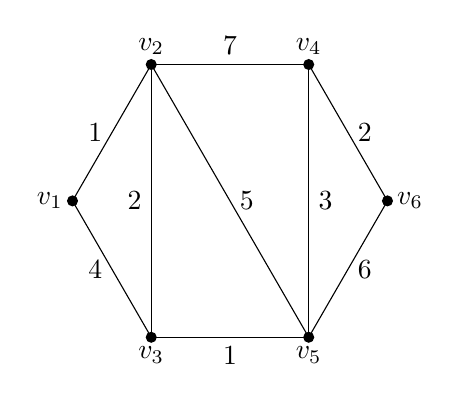
\begin{tikzpicture}
			\fill(0,0)coordinate(v1)node[left]{$v_1$}circle(2pt);
			\fill(1,{sqrt(3)})coordinate(v2)node[above]{$v_2$}circle(2pt);
			\fill(1,{-sqrt(3)})coordinate(v3)node[below]{$v_3$}circle(2pt);
			\fill(3,{sqrt(3)})coordinate(v4)node[above]{$v_4$}circle(2pt);
			\fill(3,{-sqrt(3)})coordinate(v5)node[below]{$v_5$}circle(2pt);
			\fill(4,0)coordinate(v6)node[right]{$v_6$}circle(2pt);
			\draw(v1)--(v2)node[midway,left]{1};
			\draw(v1)--(v3)node[midway,left]{4};
			\draw(v2)--(v3)node[midway,left]{2};
			\draw(v2)--(v4)node[midway,above]{7};
			\draw(v2)--(v5)node[midway,right]{5};
			\draw(v3)--(v5)node[midway,below]{1};
			\draw(v4)--(v5)node[midway,right]{3};
			\draw(v4)--(v6)node[midway,right]{2};
			\draw(v5)--(v6)node[midway,right]{6};
		\end{tikzpicture}
		\caption{}
		\label{figure:图论.边赋权无向图1}
	\end{subfigure}
	\caption{}
\end{figure}

我们可以改进邻接矩阵,用它来表示赋权图.
\begin{itemize}
	\item 如果\(v_i\)与\(v_j\)邻接,具体分为以下两种情况:\begin{itemize}
		\item 当\(G\)是赋权有向图时,
		则\(a_{ij}\)表示以\(v_i\)为起点、\(v_j\)为终点的有向边的权;
		\item 当\(G\)是赋权无向图时,
		\(a_{ij},a_{ji}\)均表示以\(v_i,v_j\)为端点的无向边的权.
	\end{itemize}
	\item 如果\(v_i\)与\(v_j\)不邻接,
	令\(a_{ij} = +\infty\).
\end{itemize}


\subsection{最短路径}
在边赋权图\(G = (V,E)\)中,
从一个顶点到另一个顶点,
路上所有边的权之和,
称为这条路的权.

例如,在\cref{figure:图论.边赋权有向图1} 中,
路\(v_2 v_3 v_5 v_6 v_7\)的权为\(2+3+1+5=11\).

从一个顶点\(v_1\)到另一个顶点\(v_2\)的、权最小的一条路,
称为“从\(v_1\)到\(v_2\)的\DefineConcept{最短路径}”.

\section{欧拉图}
欧拉图是欧拉于1736年研究七桥问题时考虑的一种图,由此得名.
\begin{definition}
%@see: 《离散数学》(邓辉文) P191 定义7-1
设\(G = (V,E)\)是图.
\begin{itemize}
	\item \(G\)中经过所有边一次且仅一次的路,
	称为\DefineConcept{欧拉轨迹}(Eulerian trail)
	或\DefineConcept{欧拉路}.

	\item \(G\)中经过所有边一次且仅一次的回路,
	称为\DefineConcept{欧拉回路}(Eulerian circuit).

	\item 存在欧拉回路的图,称为\DefineConcept{欧拉图}(Eulerian graph).
\end{itemize}
\end{definition}

显然,欧拉回路是欧拉轨迹,但欧拉轨迹不一定是欧拉回路.

\begin{theorem}[欧拉定理]
%@see: 《离散数学》(邓辉文) P191 定理7-1(欧拉定理)
设\(G\)是非平凡连通无向图,
则\(G\)是欧拉图的充分必要条件是
\(G\)的每个顶点的度数均为偶数.
%TODO proof
\end{theorem}

欧拉定理给出了一个连通图存在欧拉回路的充分必要条件.
于是接下来的问题就成了要如何具体找出一条这样的回路.
1921年 Fleury 给出了一个求解欧拉回路的算法.
%TODO

下面再介绍几个定理,它们都类似于欧拉定理.
\begin{theorem}
%@see: 《离散数学》(邓辉文) P192 定理7-2
设\(G\)是弱连通图,
则\(G\)是欧拉图的充分必要条件是
\(G\)中每个顶点的入度等于出度.
%TODO proof
\end{theorem}

\begin{example}
%@see: 《离散数学》(邓辉文) P192 例7-1
设\(G_1,G_2\)是\(n\)阶完全图\(K_n\ (n\geq4)\)的两个不同的子图.
若\(G_1,G_2\)都是欧拉图,
则\(G_1\)和\(G_2\)的对称差\(G_1 \symdiff G_2\)的每一个连通分量都是欧拉图.
%TODO proof
\end{example}

\begin{corollary}
%@see: 《离散数学》(邓辉文) P192 定理7-3
设\(G\)是连通无向图,
则\(G\)中存在欧拉轨迹的充分必要条件是
\(G\)中度数为奇数的顶点个数要么是\(0\)要么是\(2\).
%TODO proof
\end{corollary}

由上述推论可知,七桥问题无解,
在\cref{figure:图论.七桥问题} 中不存在欧拉轨迹.

\begin{theorem}
%@see: 《离散数学》(邓辉文) P192 定理7-4
设\(G\)是弱连通图,
则\(G\)中存在欧拉轨迹的充分必要条件是
\(G\)中每个顶点的入度等于出度.
%TODO proof
\end{theorem}

\begin{theorem}
%@see: 《离散数学》(邓辉文) P192 定理7-4
设\(G\)是弱连通图,
则\(G\)中存在欧拉轨迹的充分必要条件是:\begin{itemize}
	\item \(G\)中存在一个顶点\(v_1\)满足\(\degEx v_1 - \degIn v_1 = 1\);
	\item \(G\)中存在一个顶点\(v_2\)满足\(\degIn v_2 - \degEx v_2 = 1\);
	\item 除了\(v_1,v_2\)以外的其余每一个顶点\(v\)都满足\(\degEx v = \degIn v\).
\end{itemize}
%TODO proof
\end{theorem}

%TODO
% 中国邮递员问题(Chinese postman problem)
% 假设一位邮递员从邮局选好邮件去投递,然后返回邮局,
% 要求该邮递员必须经过他负责的每一条街至少一次,
% 要为他设计一条路线,使得总路程最短.
% 该问题的本质是,在允许添加多重边的情况下,在边赋权图中,求最短欧拉回路的问题.
% 该问题首次由管梅谷于1962年提出并研究,他提出了“奇偶点图上作业法”.
% 1973年,匈牙利数学家 Edmonds 和 Johnson 对中国邮递员问题给出了一种有效算法.
% 1995年,王树禾研究了多邮递员中国邮路问题(k-Postman Chinese postman problem).

\section{哈密顿图}
\begin{definition}
%@see: 《离散数学》(邓辉文) P194 定义7-2
设\(G = (V,E)\)是图.
\begin{itemize}
	\item \(G\)中经过所有顶点一次且仅一次的路径,
	称为\DefineConcept{哈密顿路径}(Hamiltonian path).

	\item \(G\)中经过所有顶点一次且仅一次(除起点重复一次外)的圈,
	称为\DefineConcept{哈密顿回路}(Hamiltonian cycle)
	或\DefineConcept{哈密顿环}%
	或\DefineConcept{哈密顿圈}.

	\item 存在哈密顿回路的图,
	称为\DefineConcept{哈密顿图}(Hamiltonian graph).
\end{itemize}
\end{definition}

显然,由哈密顿回路可以得到哈密顿路径,不返回出发点即可,
但是,反过来一般不成立.
在\cref{figure:图论.哈密顿路径1} 中,存在哈密顿路径\(bcaed\),但不存在哈密顿回路.
在\cref{figure:图论.哈密顿图1} 中,存在哈密顿回路\(v_1 v_5 v_4 v_3 v_2 v_1\),它是哈密顿图.

\begin{figure}[hbt]
%@see: 《离散数学》(邓辉文) P194 图7-8(a)
	\centering
	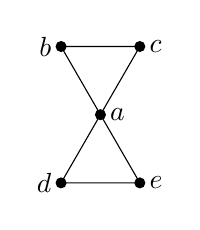
\begin{tikzpicture}
		\fill(0,0)coordinate(a)node[right]{$a$}circle(2pt);
		\fill(-.5,{.5*sqrt(3)})coordinate(b)node[left]{$b$}circle(2pt);
		\fill(.5,{.5*sqrt(3)})coordinate(c)node[right]{$c$}circle(2pt);
		\fill(-.5,{-.5*sqrt(3)})coordinate(d)node[left]{$d$}circle(2pt);
		\fill(.5,{-.5*sqrt(3)})coordinate(e)node[right]{$e$}circle(2pt);
		\draw(a)--(b)--(c)--(d)--(e)--(a);
	\end{tikzpicture}
	\caption{}
	\label{figure:图论.哈密顿路径1}
\end{figure}

\begin{figure}[hbt]
%@see: 《离散数学》(邓辉文) P194 图7-8(b)
	\centering
	\def\n{5}
	\def\b{90}
	\begin{tikzpicture}
		\pgfmathsetmacro{\m}{\n-1}
		\pgfmathsetmacro{\a}{360/\n}
		\foreach \j in {0,...,\m} {
			\fill({cos(\j*\a+\b)},{sin(\j*\a+\b)})coordinate(A\j)circle(2pt);
		}
		\draw(A0)node[above]{$v_1$}
			(A1)node[left]{$v_2$}
			(A2)node[below]{$v_3$}
			(A3)node[below]{$v_4$}
			(A4)node[right]{$v_5$};
		\begin{scope}[-{Latex[length=3mm,width=0pt 10]}]
			\draw(A0)--(A2);
			\draw(A0)--(A3);
			\draw(A0)--(A4);
			\draw(A1)--(A0);
			\draw(A2)--(A1);
			\draw(A2)--(A4);
			\draw(A3)--(A2);
			\draw(A3)--(A1);
			\draw(A4)--(A3);
			\draw(A4)--(A1);
		\end{scope}
	\end{tikzpicture}
	\caption{}
	\label{figure:图论.哈密顿图1}
\end{figure}

显然,
一个无向哈密顿图是连通图,
一个有向哈密顿图是强连通图.

\begin{theorem}
%@see: 《离散数学》(邓辉文) P195 定理7-5
设\(G = (V,E)\)是无向哈密顿图,
则\begin{equation*}
	(\forall W)
	[
		\emptyset \neq W \subset V
		\implies
		w(G-W) \leq \abs{W}
	].
\end{equation*}
%TODO proof
\end{theorem}

\begin{example}
%@see: 《离散数学》(邓辉文) P195 例7-3
举例说明:无向图\(G = (V,E)\)满足\begin{equation*}
	(\forall W)
	[
		\emptyset \neq W \subset V
		\implies
		w(G-W) \leq \abs{W}
	],
\end{equation*}
但不是哈密顿图.
%TODO 彼得森图
\end{example}

1960年,Ore得到一个哈密顿图的充分条件.
\begin{theorem}
%@see: 《离散数学》(邓辉文) P195 定理7-6(Ore,1960)
设\(G = (V,E)\)是\(n\ (n\geq3)\)阶简单无向图.
若\begin{equation*}
	(\forall u,v \in V)
	\left[
		\text{$u$与$v$不邻接}
		\implies
		\deg u + \deg v \geq n
	\right],
\end{equation*}
则\(G\)是哈密顿图.
%TODO proof
\end{theorem}

\begin{example}
%@see: 《离散数学》(邓辉文) P196 例7-4
举例说明:\(n\ (n\geq3)\)阶简单无向图\(G = (V,E)\)不满足\begin{equation*}
	(\forall u,v \in V)
	\left[
		\text{$u$与$v$不邻接}
		\implies
		\deg u + \deg v \geq n
	\right],
\end{equation*}
但它是哈密顿图.
%TODO
\end{example}

Ore的上述成果推广了Dirac于1952年给出的结果.
\begin{corollary}
%@see: 《离散数学》(邓辉文) P196 推论(Dirac,1952)
设\(G = (V,E)\)是\(n\ (n\geq3)\)阶简单无向图.
若\begin{equation*}
	(\forall v \in V)
	[\deg v \geq n/2],
\end{equation*}
则\(G\)是哈密顿图.
%TODO proof
\end{corollary}

\begin{theorem}
%@see: 《离散数学》(邓辉文) P196 定理7-7
设\(G = (V,E)\)是\(n\ (n\geq3)\)阶无向图.
若\begin{equation*}
	(\forall u,v \in V)
	\left[
		\text{$u$与$v$不邻接}
		\implies
		\deg u + \deg v \geq n-1
	\right],
\end{equation*}
则\(G\)中存在哈密顿路径.
%TODO proof
\end{theorem}

\begin{example}
%@see: 《离散数学》(邓辉文) P196 例7-5
设\(G = (V,E)\)是\(n\ (n\geq3)\)阶连通无向图.
证明:\(G\)中存在两个顶点\(u,v\),
将它们删除后得到的图\(G-\{u,v\}\)仍是连通的.
%TODO proof
\end{example}

%TODO
% 旅行商问题(travelling salesman problem)/货郎担问题
% 假设有\(n\)个城镇,其中任意两个城镇之间都有道路.
% 一个售货员要去这\(n\)个城镇售货,
% 从某城镇出发,依次访问其余\(n-1\)个城镇,
% 且每个城镇只能访问一次,最后又回到原出发地.
% 问售货员要如何安排经过\(n\)个城镇的旅行路线,
% 才能使他经过的路程最短.
% 该问题的本质是,在一个边赋权图中,找出一条权最小的哈密顿回路.
% 这是一个比判断一个图是否哈密顿图更困难的的问题.
% 当然,如果给定的赋权图是一个3阶以上的完全无向图,则哈密顿回路的存在性是显然的.
% 要求解这个问题,可以先将所有哈密顿回路找出来,再比较它们的权的大小,求出权最小的哈密顿回路即可.
% 但是对于阶数较大的赋权图来说,这样做的计算量太大.
% 求旅行商问题的近似解有“近似法”和“交换法”.
% 除此以外,人们还在研究利用遗传算法、模拟退货算法、神经网络、蚁群算法以及粒子群算法等算法.

\section{无向树}
\begin{definition}
%@see: 《离散数学》(邓辉文) P198 定义7-3
不含有圈的连通无向图,称为\DefineConcept{无向树}(tree),简称为\DefineConcept{树}.
\end{definition}

含有\(n\ (n\geq1)\)个顶点的树,称为 \DefineConcept{\(n\)阶树}.
不含顶点的树,称为\DefineConcept{空树}.

\begin{property}
%@see: 《离散数学》(邓辉文) P199 性质1
\(n\ (n\geq1)\)阶树恰有\(n-1\)条边.
%TODO proof
\end{property}

\begin{property}
%@see: 《离散数学》(邓辉文) P199 性质2
\(n\ (n\geq2)\)阶树至少有2个度为\(1\)的顶点.
%TODO proof
\end{property}

\begin{theorem}
%@see: 《离散数学》(邓辉文) P199 定理7-8
设\(G = (V,E)\)是\((n,m)\)无向图,
则\begin{align*}
	&\text{$G$是一棵树} \\
	&\iff \text{$G$不含有圈} \quad\land\quad m=n-1 \\
	&\iff \text{$G$是连通图} \quad\land\quad m=n-1 \\
	&\iff \text{$G$不含有圈,但新增一条边后成为一个圈} \\
	&\iff \text{$G$是连通图,但删除任意一条边后成为非连通图} \\
	&\iff \text{$G$的每一对顶点有且仅有一条路径}.
\end{align*}
%TODO proof
\end{theorem}

\begin{definition}
%@see: 《离散数学》(邓辉文) P200 定义7-4
设\(G = (V,E)\)是无向图.
若\(G\)的生成子图\(T\)是树,
则称“\(T\)是\(G\)的\DefineConcept{生成树}(spanning tree)”.
\end{definition}

\cref{figure:图论.生成树.无向图1} 所示的无向图不是树,
但它的生成子图 \labelcref{figure:图论.生成树.无向图1的生成树1,figure:图论.生成树.无向图1的生成树2} 是树.

\begin{figure}[hbt]
%@see: 《离散数学》(邓辉文) P200 图7-21
	\centering
	\def\subwidth{.3\linewidth}
	\begin{subfigure}[b]{\subwidth}
		\centering
		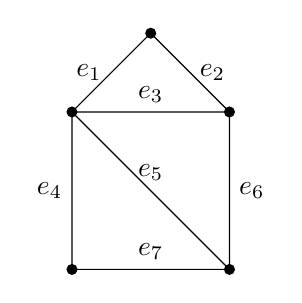
\begin{tikzpicture}
			\fill(0,0)coordinate(v1)circle(2pt);
			\fill(2,0)coordinate(v2)circle(2pt);
			\fill(2,2)coordinate(v3)circle(2pt);
			\fill(1,3)coordinate(v4)circle(2pt);
			\fill(0,2)coordinate(v5)circle(2pt);
			\draw(v3)--(v4)node[midway,right]{$e_2$}
				--(v5)node[midway,left]{$e_1$}
				--(v1)node[midway,left]{$e_4$}
				--(v2)node[midway,above]{$e_7$}
				--(v3)node[midway,right]{$e_6$}
				--(v5)node[midway,above]{$e_3$}
				--(v2)node[midway,above]{$e_5$};
		\end{tikzpicture}
		\caption{}
		\label{figure:图论.生成树.无向图1}
	\end{subfigure}~\begin{subfigure}[b]{\subwidth}
		\centering
		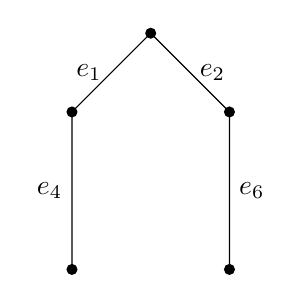
\begin{tikzpicture}
			\fill(0,0)coordinate(v1)circle(2pt);
			\fill(2,0)coordinate(v2)circle(2pt);
			\fill(2,2)coordinate(v3)circle(2pt);
			\fill(1,3)coordinate(v4)circle(2pt);
			\fill(0,2)coordinate(v5)circle(2pt);
			\draw(v2)--(v3)node[midway,right]{$e_6$}
				--(v4)node[midway,right]{$e_2$}
				--(v5)node[midway,left]{$e_1$}
				--(v1)node[midway,left]{$e_4$};
		\end{tikzpicture}
		\caption{}
		\label{figure:图论.生成树.无向图1的生成树1}
	\end{subfigure}~\begin{subfigure}[b]{\subwidth}
		\centering
		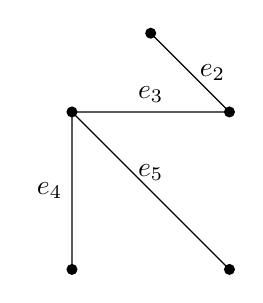
\begin{tikzpicture}
			\fill(0,0)coordinate(v1)circle(2pt);
			\fill(2,0)coordinate(v2)circle(2pt);
			\fill(2,2)coordinate(v3)circle(2pt);
			\fill(1,3)coordinate(v4)circle(2pt);
			\fill(0,2)coordinate(v5)circle(2pt);
			\draw(v4)--(v3)node[midway,right]{$e_2$}
				--(v5)node[midway,above]{$e_3$}
				--(v1)node[midway,left]{$e_4$}
				(v5)--(v2)node[midway,above]{$e_5$};
		\end{tikzpicture}
		\caption{}
		\label{figure:图论.生成树.无向图1的生成树2}
	\end{subfigure}
	\caption{}
\end{figure}

不是每一个无向图都有生成树.
即便某个无向图有生成树,它的生成树也不一定唯一.

\begin{theorem}
%@see: 《离散数学》(邓辉文) P201 定理7-9
设\(G\)是无向图,
则\(G\)有生成树的充分必要条件是\(G\)是连通图.
%TODO proof
\end{theorem}

\begin{corollary}
%@see: 《离散数学》(邓辉文) P201 推论
\(n\ (n\geq1)\)阶连通图至少有\(n-1\)条边.
\end{corollary}

\begin{corollary}
%@see: 《离散数学》(邓辉文) P201
\(n\ (n\geq1)\)阶树是边数最少的连通无向图.
\end{corollary}

\begin{example}
%@see: 《离散数学》(邓辉文) P201 例7-8
设\(G\)是连通无向图,
\(T\)是\(G\)的任意一棵生成树,
\(C\)是\(G\)的任意圈,
则\(C\)至少含有一条关于生成树\(T\)中的弦.
%TODO 什么是弦???未定义!
%TODO proof
\end{example}

\begin{example}
%@see: 《离散数学》(邓辉文) P201 例7-9
设\(G\)是连通无向图,
\(T\)是\(G\)的任意一棵生成树,
\(F\)是\(G\)的任意一个边割集,
则\(F\)至少有一条\(T\)中的树枝.
%TODO 什么是树枝???未定义!
%TODO proof
\end{example}

\begin{definition}
%@see: 《离散数学》(邓辉文) P201 定义7-5
设\(G\)是一个边赋权的连通无向图,
\(G\)的生成树\(T\)的各边的权之和,
称为“\(T\)的\DefineConcept{权}”.
\(G\)的权最小的生成树,
称为“\(G\)的\DefineConcept{最小生成树}(minimal spanning tree)”.
\end{definition}

\section{有向树,根树}
\subsection{有向树}
\begin{definition}
%@see: 《离散数学》(邓辉文) P203 定义7-6
设\(G = (V,E)\)是有向图.
若\(G\)的基础图是一棵树,
则称“\(G\)是一棵\DefineConcept{有向树}(directed tree)”.
\end{definition}

\begin{definition}
%@see: 《离散数学》(邓辉文) P203
设\(G\)是有向树,结点\(v \in G\).
\begin{itemize}
	\item \(v\)的前趋元素,称为“\(v\)的\DefineConcept{父结点}(parent)”.
	\item \(v\)的后继元素,称为“\(v\)的\DefineConcept{子结点}(child)”.
\end{itemize}
\end{definition}

\subsection{根树}
\begin{definition}
%@see: 《离散数学》(邓辉文) P203 定义7-7
若有向树\(T\)恰有1个结点入度为\(0\),而其余结点入度均为\(1\),
则称“\(T\)是一棵\DefineConcept{根树}(rooted tree)”.
\end{definition}

\begin{definition}
%@see: 《离散数学》(邓辉文) P203
设\(T\)是根树.
\begin{itemize}
	\item 将\(T\)中入度为\(0\)的结点称为“\(T\)的\DefineConcept{根结点}(root)”.
	\item 将\(T\)中出度为\(0\)的结点称为“\(T\)的\DefineConcept{叶子结点}(leaf)”.
	\item 将\(T\)中出度大于\(0\)的结点称为“\(T\)的\DefineConcept{分支结点}”.
	\item 将\(T\)中除了根结点以外的分支结点称为“\(T\)的\DefineConcept{内部结点}”.
\end{itemize}
\end{definition}

\begin{definition}
%@see: 《离散数学》(邓辉文) P203
设\(T\)是根树,结点\(v \in T\).
\begin{itemize}
	\item 如果结点\(u \in T\)和\(v\)的父结点相同,
	则称“\(u\)是\(v\)的\DefineConcept{兄弟结点}(sibling)”.
	\item 从根结点到\(v\)的路径上所经过的所有分支结点,
	%TODO 为什么“祖先”的定义要以“分支结点”为基础?
	%TODO \(v\)的祖先是否包括\(v\)自己,难不成根据\(v\)是叶子结点还是分支结点,还要进一步讨论?
	%TODO 我估计这里默认在讨论结点\(v\)的祖先时,是把这个结点当做叶子结点来看待的,那就不应该包括它.
	称为“\(v\)的\DefineConcept{祖先}(ancestor)”.
	\item \(v\)可达的全体结点,
	称为“\(v\)的\DefineConcept{后代}(offspring, descendants)”.
\end{itemize}
\end{definition}

可以证明,在根树中,从根结点到任意一个结点,有且仅有一条路径.

\begin{definition}
%@see: 《离散数学》(邓辉文) P204
设\(T\)是根树,结点\(v \in T\).
从根结点到\(v\)的路径的路长,
称为“\(v\)的\DefineConcept{层次}(level)”.
如果\(v\)的层次等于\(l\),
则称“\(v\)是第\(l\)层结点”.
\end{definition}

由定义有,根结点是第\(0\)层结点,根结点的子结点(如若存在)就是第\(1\)层结点,以此类推.

\begin{definition}
%@see: 《离散数学》(邓辉文) P204
设\(T\)是根树,结点\(u,v,u',v' \in T\),
\(u'\)是\(u\)的父结点,\(v'\)是\(v\)的父结点.
如果\(u'\)的层次等于\(v'\)的层次,
则称“\(u\)是\(v\)的\DefineConcept{堂兄弟结点}(cousin)”.
\end{definition}

\begin{definition}
%@see: 《离散数学》(邓辉文) P204
设\(T\)是根树.
\(T\)中各个结点的层次的最大值,
称为“\(T\)的\DefineConcept{深度}(depth)”
或“\(T\)的\DefineConcept{高度}(height)”.
\end{definition}

\begin{definition}
%@see: 《离散数学》(邓辉文) P204
设\(T\)是根树.
\begin{itemize}
	\item \(T\)的所有叶子结点的层次之和,称为\(T\)的\DefineConcept{外部路径长度}.
	\item \(T\)的所有内部结点的层次之和,称为\(T\)的\DefineConcept{内部路径长度}.
\end{itemize}
\end{definition}

\begin{definition}
%@see: 《离散数学》(邓辉文) P204 定义7-8
设\(G = (V,E)\)是一棵根树,结点\(v \in V\).
由结点\(v\)及其所有后代导出的子图,
称为“\(G\)的\DefineConcept{子根树}(rooted subtree)”,
简称为\DefineConcept{子树}(subtree).
\end{definition}

\subsection{多叉树}
\begin{definition}
%@see: 《离散数学》(邓辉文) P204 定义7-9
设\(G = (V,E)\)是一棵根树.
若\(\max_{v \in V} \degEx v = m\),
则称“\(G\)是一棵 \DefineConcept{\(m\)叉树}”.
\end{definition}

\begin{definition}
%@see: 《离散数学》(邓辉文) P204
设\(T\)是\(m\)叉树.
\begin{itemize}
	\item 若对于任意结点\(v\),均有\(\degEx v = m\)或\(\degEx v = 0\),
	则称“\(G\)是\DefineConcept{完全\(m\)叉树}”.

	\item 所有叶子结点的层次都相同的完全\(m\)叉树,
	称为\DefineConcept{正则\(m\)叉树}或\DefineConcept{满\(m\)叉树}.
\end{itemize}
\end{definition}

\begin{property}
%@see: 《离散数学》(邓辉文) P204 性质1
\(m\)叉树的第\(i\)层至多有\(m^i\)个结点.
%TODO proof
\end{property}

\begin{property}
%@see: 《离散数学》(邓辉文) P204 性质2
高度为\(h\)的\(m\ (m\geq2)\)叉树至多有\(\frac{m^{h+1}-1}{m-1}\)个结点.
%TODO proof
\end{property}

\begin{property}
%@see: 《离散数学》(邓辉文) P204 性质3
一棵有\(l\)个叶子结点的\(m\)叉树的高度至少为\(\log_m l\).
%TODO proof
\end{property}

\begin{property}
%@see: 《离散数学》(邓辉文) P204 性质4
若一棵完全\(m\)叉树有\(l\)个叶子结点、\(t\)个分支结点,
则\begin{equation*}
	(m-1)t=l-1.
\end{equation*}
%TODO proof
\end{property}

\begin{property}
%@see: 《离散数学》(邓辉文) P204 性质5
若二叉树有\(l\)个叶子结点,则出度为\(2\)的结点有\(l-1\)个.
%TODO proof
\end{property}

\begin{property}
%@see: 《离散数学》(邓辉文) P204 性质6
有\(l\)个叶子结点的完全二叉树有\(2l-1\)个结点.
%TODO proof
\end{property}

\begin{property}
%@see: 《离散数学》(邓辉文) P204 性质7
若完全二叉树有\(t\)个分支结点,
则它的外部路径长度\(E\)与它的内部路径长度\(I\)满足\begin{equation*}
	E = I + 2t.
\end{equation*}
%TODO proof
\end{property}

\subsection{叶赋权多叉树,哈夫曼树}
\begin{definition}
%@see: 《离散数学》(邓辉文) P205 定义7-10
设\(G = (V,E)\)是一棵\(m\)叉树,
映射\(\omega\colon W \to \mathbb{R}\),
其中\(W\)是\(G\)的全体叶子结点,
则称“\((G,\omega)\)是\DefineConcept{叶赋权\(m\)叉树}”,
把\(\omega\)称为“\(G\)的\DefineConcept{叶子赋权映射}”.
\end{definition}

叶赋权\(m\)叉树给它的每一个叶子结点都赋予了一个非负实数权.

\begin{definition}
%@see: 《离散数学》(邓辉文) P205 定义7-11
设\(G = (V,E)\)是一棵叶赋权\(m\)叉树,
其全部\(l\)个叶子结点上的权分别是\begin{equation*}
	w_i
	\quad(i=1,2,\dotsc,l).
\end{equation*}
将从根结点到权为\(w_i\)的叶子结点的路径的路长
分别记为\begin{equation*}
	L(w_i)
	\quad(i=1,2,\dotsc,l).
\end{equation*}
把\begin{equation*}
	\sum_{i=1}^l w_i \cdot L(w_i)
\end{equation*}称为“\(G\)的\DefineConcept{权}”,
记为\(W(G)\).
对于任意一个叶子结点\(v \in W\),
把\(\omega(v)\)称为“\(v\)的\DefineConcept{权}(weight)”.
\end{definition}

\begin{definition}
%@see: 《离散数学》(邓辉文) P206 定义7-12
设\begin{equation*}
	\mathcal{T}
	\defeq
	\Set{
		T \given \text{$T$是一棵叶赋权二叉树,其$l$个叶子结点上的权分别是$\AutoTuple{w}{l}$}
	},
\end{equation*}
把\(\mathcal{T}\)中权最小的那棵叶赋权二叉树
称为\DefineConcept{最优二叉树}
或\DefineConcept{哈夫曼树}(Huffman tree).
\end{definition}

\subsection{有序树}
在根树的定义中,同一个结点的不同子结点之间是没有先后顺序的,这与现实生活中的家族树不一样.
当我们需要考虑兄弟结点之间的先后顺序时,我们就要用到“有序树”了.
\begin{definition}
%@see: 《离散数学》(邓辉文) P207 定义7-13
设\(G = (V,E)\)是一棵根树.
若对每一个结点的所有子结点都规定了先后顺序,
则称“\(G\)是一棵\DefineConcept{有序树}(ordered tree)”.
\end{definition}

\subsection{定位二叉树}
\begin{definition}
%@see: 《离散数学》(邓辉文) P207 定义7-14
设\(G = (V,E)\)是一棵有序二叉树.
若对每一个结点的所有儿子结点规定一个左右位置,
则称“\(G\)是一棵\DefineConcept{定位二叉树}(positional binary tree)”.
\end{definition}

\section{平面图}
\subsection{平面图的定义}
%@see: 《离散数学》(邓辉文) P211 定义7-16
设\(G\)是无向图.
如果可以将\(G\)画在一个平面上,
同时使得任意两条相异边在非端点处不相交,
则称“\(G\)是一个\DefineConcept{平面图}(planar graph)”.

设\(G\)是平面图,
\(G\)的图形表示如果可以画在一个平面上,
同时使得任意两条相异边在非端点处不相交,
则称其为“\(G\)的\DefineConcept{平面嵌入}(planar embedding)”
或“\(G\)的\DefineConcept{平面表示}”.

\begin{definition}
%@see: 《离散数学》(邓辉文) P211 定义7-17
设\(G\)是简单平面图.
若在\(G\)的任意两个不相邻的顶点\(u\)和\(v\)之间增加一条边,
所得到的图\(G+uv\)是非平面图,
则称“\(G\)是一个\DefineConcept{极大平面图}(maximal planar graph)”.
\end{definition}

\begin{definition}
%@see: 《离散数学》(邓辉文) P211 定义7-18
设\(G\)是非平面图.
若在\(G\)中任意删除一条边,所得到的图是平面图,
则称“\(G\)是一个\DefineConcept{极小非平面图}(minimal nonplanar graph)”.
\end{definition}

\begin{definition}
%@see: 《离散数学》(邓辉文) P211 定义7-19
设\(G\)是平面图.
由\(G\)的若干条边所围成的连通\footnote{
	一个区域是连通的,是指“在其内部可以随意走动而不必穿过任何一条边”.
}区域,
%TODO 这个定义似乎很不严谨,需要忖度一下如何重新表述
称为“\(G\)的一个\DefineConcept{面}(face)”,
围成面的回路称为这个面的\DefineConcept{边界}(boundary).
\end{definition}
\begin{remark}
任何一个平面图都有一个由若干条边向外围成的一个面,它是唯一一个无限面.
\end{remark}

平面图的两个面相邻,是指这两个面有公共边界.

\subsection{欧拉公式}
\begin{theorem}
%@see: 《离散数学》(邓辉文) P212 定理7-10(欧拉公式)
任意\((n,m)\)连通无向图的面数\(r\)满足\begin{equation}
	r = m - n + 2.
\end{equation}
%TODO proof
\end{theorem}
\begin{remark}
在欧拉公式中,“连通”这一条件是必不可少的.
\end{remark}

\begin{corollary}
%@see: 《离散数学》(邓辉文) P212 推论1
对于任意\((n,m)\)简单连通平面图\(G\),有\begin{equation*}
	n\geq3 \implies m\leq3n-6.
\end{equation*}
%TODO proof
\end{corollary}

\begin{example}
%@see: 《离散数学》(邓辉文) P212 例7-16
证明:\(K_5\)不是平面图.
%TODO proof
\end{example}

\begin{corollary}
%@see: 《离散数学》(邓辉文) P212 推论2
对于任意\((n,m)\)简单连通平面图\(G\),
若\(G\)不含\(K_3\)子图,且\(n\geq3\),
则\(m\leq2n-4\).
%TODO proof
\end{corollary}

\begin{example}
%@see: 《离散数学》(邓辉文) P212 例7-17
证明:\(K_{3,3}\)不是平面图.
%TODO proof
\end{example}

\begin{theorem}
%@see: 《离散数学》(邓辉文) P212 定理7-11
任何简单平面图必有一个度数小于等于\(5\)的顶点.
%TODO proof
\end{theorem}

\subsection{库拉托夫斯基定理}
波兰数学家库拉托夫斯基于1930年给出了判定平面的充分必要条件.

\begin{theorem}
%@see: 《离散数学》(邓辉文) P213 定理7-12(Kuratowski, 1930)
无向图\(G\)是平面图的充分必要条件是:
\(G\)没有同胚于\(K_5\)和\(K_{3,3}\)的子图.
%TODO proof
\end{theorem}

\begin{example}
%@see: 《离散数学》(邓辉文) P213
证明:彼得森图不是平面图.
%TODO proof
\end{example}

\subsection{平面图的对偶图}
对平面图的面的研究,可以转换为对其对偶图的顶点的研究.
\begin{definition}
%@see: 《离散数学》(邓辉文) P213 定义7-21
设\(G\)是平面图.
\(G\)的\DefineConcept{对偶图}(记作\(G^*\))构造如下:\begin{itemize}
	\item 在\(G\)的每一个面内取一个点,作为\(G^*\)的顶点;
	\item 若\(G\)内的两个面有公共边界\(e\),
	则在\(G^*\)中将这两个面对应的顶点连接起来得到一条边\(e^*\),
	使得\(e^*\)与\(e\)相交一次而与\(G\)的其余边不相交.
	若\(e\)是\(G\)的桥,
	则\(e^*\)是\(G^*\)的吊环.
	若\(e\)是\(G\)的吊环,
	则\(e^*\)是\(G^*\)的桥.
%TODO 什么是吊环???未定义!
\end{itemize}
\end{definition}

%@see: 《离散数学》(邓辉文) P214
根据定义可知,任意平面图的对偶图都是连通平面图.

%@see: 《离散数学》(邓辉文) P214
设\(G\)是\((n,m)\)平面图,有\(r\)个面,则\(G^*\)是\((r,m)\)平面图,有\(n\)个面.

%@see: 《离散数学》(邓辉文) P214
连通平面图\(G\)的对偶图\(G^*\)的对偶图\(G^{**}\)就是\(G\)本身.
非联通平面图\(G\)的对偶图\(G^*\)的对偶图\(G^{**}\)可能与\(G\)不同构.


\endgroup
